\documentclass[12pt,oneside,a4paper,brazil]{abntex2}
\usepackage[utf8]{inputenc}
\usepackage[T1]{fontenc}
\usepackage{lmodern,microtype,indentfirst,graphicx,url,enumitem,float}
\usepackage{longtable,array,amsmath,xurl,tikz}
\usepackage{hyperref}
\hypersetup{hypertexnames=false}
\graphicspath{{imgs/}}
\titulo{ponto-a-ponto: Deslocamento facilitado entre origem e destino.}
\autor{André Meneghelli Vale \\ Ariana Harumi Uemura \\ Bruno Gabriel Migliari de Souza \\ Caio Wellington Procopio Ferreira \\ Ingrid Emanuelle Sousa Dias \\ Leonardo Souza Leite \\ Maurício Gonçalves Marques}
\local{São Bernardo do Campo; Suzano; Francisco Morato; Osasco -- SP}
\data{2026}
\instituicao{Universidade Virtual do Estado de São Paulo -- UNIVESP}
\tipotrabalho{Relatório Técnico-Científico Parcial}
\preambulo{Relatório parcial apresentado à disciplina de Projeto Integrador em Computação II. Orientadora: Me. Aline Monteiro Campos Garcia.}
\begin{document}
\selectlanguage{brazil}\frenchspacing
\imprimircapa
\begin{resumo}
Este projeto desenvolve o ponto-a-ponto, aplicação web que associa um QR Code à parada para ampliar as informações disponíveis no ponto de ônibus. O acesso pelo navegador identifica a origem sem exigir conhecimento prévio do nome da parada, de seu endereço ou das linhas, nem instalação de aplicativo. A tese de Haylett sobre clareza da informação de viagem orienta o escopo: apoiar a compreensão do deslocamento por passageiros com diferentes graus de familiaridade com a rede, apresentando primeiro as alternativas e depois seus detalhes. O protótipo implementa backend Django/Python, frontend React, mapa Leaflet e persistência em SQLite. Utiliza OpenStreetMap e catálogos públicos complementares, preservando a procedência dos registros. O inventário reúne 1.616 registros de paradas e terminais; 172 possuem coordenadas, das quais 30 são estimativas por endereço e sentido do itinerário, ainda sem validação operacional. O planejamento aplica Dijkstra a viagens demonstrativas, considerando espera, deslocamento e baldeações. As seis linhas de demonstração, os horários e os veículos são simulados e administrados em uma página restrita; não representam previsões reais de Mauá. A interface permite selecionar destino, comparar alternativas e salvar favoritos no navegador. A avaliação com Osmar e passageiros permanece prevista e deverá observar conclusão das tarefas, compreensão de sentido e transferências, necessidade de ajuda e reconhecimento das limitações dos dados. A implantação em pontos reais depende de autorização e de validação do cadastro; integração operacional e aplicativo Android são evoluções futuras.

\par\vfill
\noindent\textbf{Palavras-chave}: transporte público; QR Code; informação ao passageiro; mobilidade urbana; pontos de interesse.
\end{resumo}
% Ajuste local do espaço do título; preserva fonte e entradas do sumário.
\begingroup
\setlength{\beforechapskip}{0pt}
\setlength{\afterchapskip}{6pt}
\setlength{\cftbeforechapterskip}{2pt}
\setlength{\cftbeforesubsectionskip}{-1.3pt}
\tableofcontents*
\endgroup
\cleardoublepage

\chapter{Introdução}
O projeto denomina-se \textbf{ponto-a-ponto} e tem como frase de apresentação \textit{``Deslocamento facilitado entre origem e destino.''} O nome sintetiza a proposta de apoiar o passageiro na escolha do percurso, desde a identificação do ponto de embarque até o destino desejado, incluindo eventuais trocas de ônibus. A frase expressa o propósito do projeto; os benefícios para os passageiros ainda deverão ser avaliados com a comunidade.

A informação em tempo real pode reduzir tempos de espera, influenciar escolhas de trajetos e aumentar a satisfação dos passageiros \cite{brakewood2019}. Este PI aborda o problema a partir do próprio ponto: o QR Code funciona como uma ligação entre o ambiente físico e informações digitais úteis à decisão de viagem. Ao ler o código, o passageiro deverá acessar no navegador uma interface que já identifica a parada e apresenta as alternativas disponíveis. O acesso inicial deverá dispensar conhecimento prévio do nome ou número da linha, do nome do ponto e de seu endereço, assim como a instalação de um aplicativo. Dessa forma, a presença do passageiro no local torna-se suficiente para definir o contexto inicial da consulta, desde que ele disponha de um celular capaz de ler o código e acessar a internet.

A motivação possui antecedente na Hackatona do Ônibus de 2013, para a qual um integrante submeteu individualmente uma proposta que não foi selecionada para a etapa presencial. O evento utilizava dados reais da SPTrans e desafios derivados das necessidades dos usuários \cite{hackatona2013}. Em notícia de 24 de junho de 2014, a Prefeitura de São Paulo descreve o acesso por QR Code à página da parada, com suas linhas e, após a escolha de uma delas, trajeto e veículos no Olho Vivo. A publicação vincula a iniciativa à Hackatona da SPTrans \cite{qrsptrans2014}. Esse registro constitui um antecedente da proposta e não comprova vínculo entre a contribuição individual mencionada e o sistema implantado.

O uso do QR Code e do ponto físico como contexto inicial é, portanto, uma abordagem já existente. A contribuição pretendida deste PI inclui a aplicação dessa abordagem ao contexto de Mauá e a construção e avaliação, com a comunidade externa, de um fluxo integrado que apresente as alternativas do ponto e permita filtrá-las pelo destino desejado. A proposta prevê a visualização conjunta dos veículos que se aproximam, destacando o mais próximo de cada linha, para permitir a comparação das alternativas sem consultas sucessivas por linha. A personalização por destinos favoritos no navegador complementa esse fluxo no protótipo. Essas funcionalidades deverão ser avaliadas, sem alegação de ineditismo ou de superioridade já demonstrada.

A proposta atual foi delimitada após interação com a comunidade externa, especialmente a conversa com Osmar, profissional com passagem pela EMTU e experiência no transporte público. Segundo o relato do grupo sobre o contexto local, Mauá não dispõe dessa forma de acesso às informações por QR Codes nos pontos de ônibus. Na conversa inicial, Osmar demonstrou entusiasmo com a ideia, o que motivou o desenvolvimento da proposta para avaliação local. A solução implementada é uma aplicação web responsiva com backend Django/Python e frontend React, baseada em dados do OpenStreetMap e em catálogos públicos complementares. A implementação técnica não equivale à validação com a comunidade.

\chapter{Desenvolvimento}
\section{Objetivos}
\subsection{Objetivo geral}
Desenvolver e avaliar um protótipo web de informação ao passageiro, acessível por QR Code no ponto de ônibus, que auxilie a compreender e escolher um deslocamento sem exigir conhecimento prévio da rede, distinguindo dados cadastrados, estimativas e simulação.

\subsection{Objetivos específicos}
\begin{enumerate}[label=\alph*)]
\item levantar necessidades de passageiros familiarizados e não familiarizados com o deslocamento, com participação da comunidade externa;
\item importar e documentar fontes públicas de paradas, linhas e itinerários, preservando identificadores, datas e limitações;
\item estimar coordenadas por endereço e sequência do itinerário, registrando incertezas e pendências para validação posterior;
\item implementar a aplicação em Django/Python e React, com SQLite e acesso contextualizado por QR Code;
\item aplicar Dijkstra a cenários controlados, incluindo espera, sentido das viagens e baldeações viáveis;
\item apresentar alternativas por destino, trajetos sobre ruas, detalhes das etapas e favoritos opcionais no navegador;
\item manter a simulação identificada e controlada exclusivamente pela administração;
\item verificar tecnicamente os fluxos e avaliar sua compreensão com Osmar e passageiros, sem confundir testes de software com validação de usabilidade; e
\item definir, com os responsáveis pela operação, os requisitos de cadastro, atualização e eventual integração de dados reais.
\end{enumerate}

\section{Justificativa e delimitação do problema}
\textbf{Pergunta de pesquisa:} \textit{Como o acesso a uma aplicação web por QR Code no ponto de ônibus pode ampliar as informações disponíveis no local e facilitar a escolha do deslocamento por passageiros sem conhecimento prévio das linhas, da identificação da parada ou de seu endereço, e sem aplicativo instalado?}

A ausência dessa tecnologia em Mauá, conforme relatada pelo grupo, constitui uma motivação local para o projeto. A existência de uma iniciativa anterior em São Paulo oferece uma referência para o desenvolvimento, enquanto a pertinência da proposta em Mauá decorre das necessidades identificadas no território e do interesse manifestado na interação com a comunidade externa.

O escopo desta etapa compreende uma aplicação web funcional, um catálogo rastreável de fontes públicas e cenários operacionais simulados para apresentação a Osmar. A contribuição central é apoiar a decisão a partir do destino, com informação compreensível sobre linhas, sentido, espera e trocas, em vez de exigir que o passageiro reconheça previamente a linha adequada. A hipótese de melhoria da compreensão deverá ser testada localmente; a literatura orienta o projeto, mas não comprova seus resultados em Mauá.

O planejamento demonstrativo e o catálogo importado são camadas distintas: possuir uma linha ou uma coordenada no banco não assegura itinerário completo, horário vigente ou conexão operacional válida. Não integram a entrega atual previsões reais de chegada, cobertura integral validada da cidade, implantação autorizada de placas, aplicativo Android ou levantamento populacional de origem e destino. Favoritos já são armazenados no navegador, sem conta nem sincronização entre dispositivos. O acesso inicial pelo QR Code permanece independente dessa personalização.

\section{Fundamentação teórica}
\subsection{Informação ao passageiro e tempo real}
Sistemas de informação ao passageiro combinam dados estáticos com informações dinâmicas como atrasos, previsões e localização. Brakewood e Watkins sintetizam evidências sobre benefícios da informação em tempo real \cite{brakewood2019}.

\subsection{GPS, AVL e localização dos veículos}
Sistemas AVL acompanham a frota por dados de posição. O GTFS-Realtime prevê posições de veículos, atualizações de viagens e alertas \cite{gtfs}. A API Olho Vivo é um exemplo brasileiro de consultas de linhas, paradas, posições e previsões por HTTP/JSON \cite{sptransapi}.

\subsection{Dados abertos e GTFS/GTFS-Realtime}
GTFS é um padrão aberto para informação de transporte. GTFS Schedule descreve paradas, rotas, viagens e horários; GTFS-Realtime complementa com atualizações, alertas e posições \cite{gtfs}. Estudos mostram aplicações de GTFS em análise e visualização de redes \cite{pereira2023,ma2020}.

\subsection{Redes de transporte e grafos}
O planejamento implementado utiliza Dijkstra sobre estados de viagens e paradas, com tempos não negativos em segundos. A prioridade é a chegada mais cedo ao destino no cenário e na janela de serviço considerados, e não a menor distância geográfica. O uso de estados temporais permite representar espera e compatibilidade entre conexões \cite{sedgewicksp,transitplanner}.

No ponto-a-ponto, o estado identifica a viagem, a posição na sequência de paradas e a quantidade de embarques. Continuar na mesma viagem não constitui baldeação. Uma troca exige outro veículo na mesma parada e partida posterior à chegada acrescida do intervalo mínimo configurado, de 120 segundos por padrão. O limite de baldeações é configurável. Transferências a pé entre paradas distintas ainda não são representadas; para um destino indicado por coordenada, admite-se caminhada final a partir de paradas até 500 metros, com velocidade suposta de 1,3 m/s. Esses parâmetros são hipóteses do cenário, não medidas de acessibilidade ou da operação local.

O resultado separa espera, tempo a bordo, caminhada final e trocas, sem duplicar intervalos. Por exemplo, cinco minutos de espera inicial, doze no primeiro veículo, quatro entre a chegada e a próxima partida e dez no segundo veículo totalizam 31 minutos e uma baldeação; o intervalo mínimo de transferência já está contido nos quatro minutos. As alternativas são ordenadas por chegada e, em caso de empate, pelo número de trocas. A consulta considera também partidas posteriores ao ônibus mais próximo, pois elas podem produzir uma chegada anterior.

Dijkstra escolhe entre os tempos fornecidos; não prevê trânsito. As seis linhas demonstrativas utilizam horários e durações simulados. O cadastro público importado permanece fora desse planejamento quando não oferece sequência, geometria e tempos suficientes. Não encontrar caminho significa ausência de conexão nos dados e na janela consultados, e não prova de inexistência de serviço real. A inclusão de tempos operacionais exigirá atualização das entradas e nova verificação das conexões.

\subsection{QR Code como interface físico-digital}
Em Southampton, QR Codes únicos foram instalados em 44 pontos para acesso a informações de chegada \cite{southampton}. O caso da SPTrans documenta o uso do QR Code junto à sinalização física, com manutenção dos informativos tradicionais. A notícia de 2014 orientava instalar um aplicativo para ler o código; essa orientação se refere ao leitor de QR Code \cite{qrsptrans2014}. Neste PI, o QR Code é concebido como uma interface que estende o ambiente real com dados úteis ao passageiro: o próprio local fornece o contexto que, em uma busca convencional, precisaria ser informado manualmente. A proposta é que o código contenha um endereço web vinculado à parada, permitindo identificá-la sem exigir que o usuário conheça seu nome, endereço ou linhas atendidas. A consulta inicial deverá ocorrer no navegador, sem cadastro obrigatório ou instalação de aplicativo específico do projeto. O acesso pressupõe que o dispositivo disponha de um recurso capaz de ler QR Codes, além de conexão à internet.

\clearpage
\subsection{QRCodeAdesivo: acesso por QR Code no ponto de ônibus}
\label{sec:analise-qrcodeadesivo}
O levantamento considera separadamente duas soluções vinculadas à SPTrans. A primeira é o QRCodeAdesivo, página de informações da parada acessada pelo QR Code instalado no ponto; a segunda é o Olho Vivo, sistema de consulta de ônibus, previsões e mapas, analisado na subseção seguinte. Embora a página do QRCodeAdesivo contenha links para o Olho Vivo, essa ligação não torna as capturas dos dois ambientes uma única sequência de uso.

O QRCodeAdesivo é um antecedente direto do acesso físico-digital proposto pelo PI. A notícia de 2014 documenta sua implantação \cite{qrsptrans2014}. O grupo levanta a hipótese de que sua evolução tenha sido descontinuada ou limitada, com base nos indícios técnicos apresentados após a captura; a hipótese não equivale à confirmação de encerramento do serviço.

\textbf{Acesso contextualizado pela leitura do QR Code.}
A página da parada 70016782, na Avenida Paulista, número 200, apresenta as linhas e os acessos individuais de localização, previsão e informações (Figura~\ref{fig:sptrans-parada}). O QR Code dispensa a digitação da origem, mas essa página não relaciona automaticamente as linhas ao destino pretendido pelo passageiro \cite{sptransparada70016782}.

\begin{figure}[H]
    \centering
    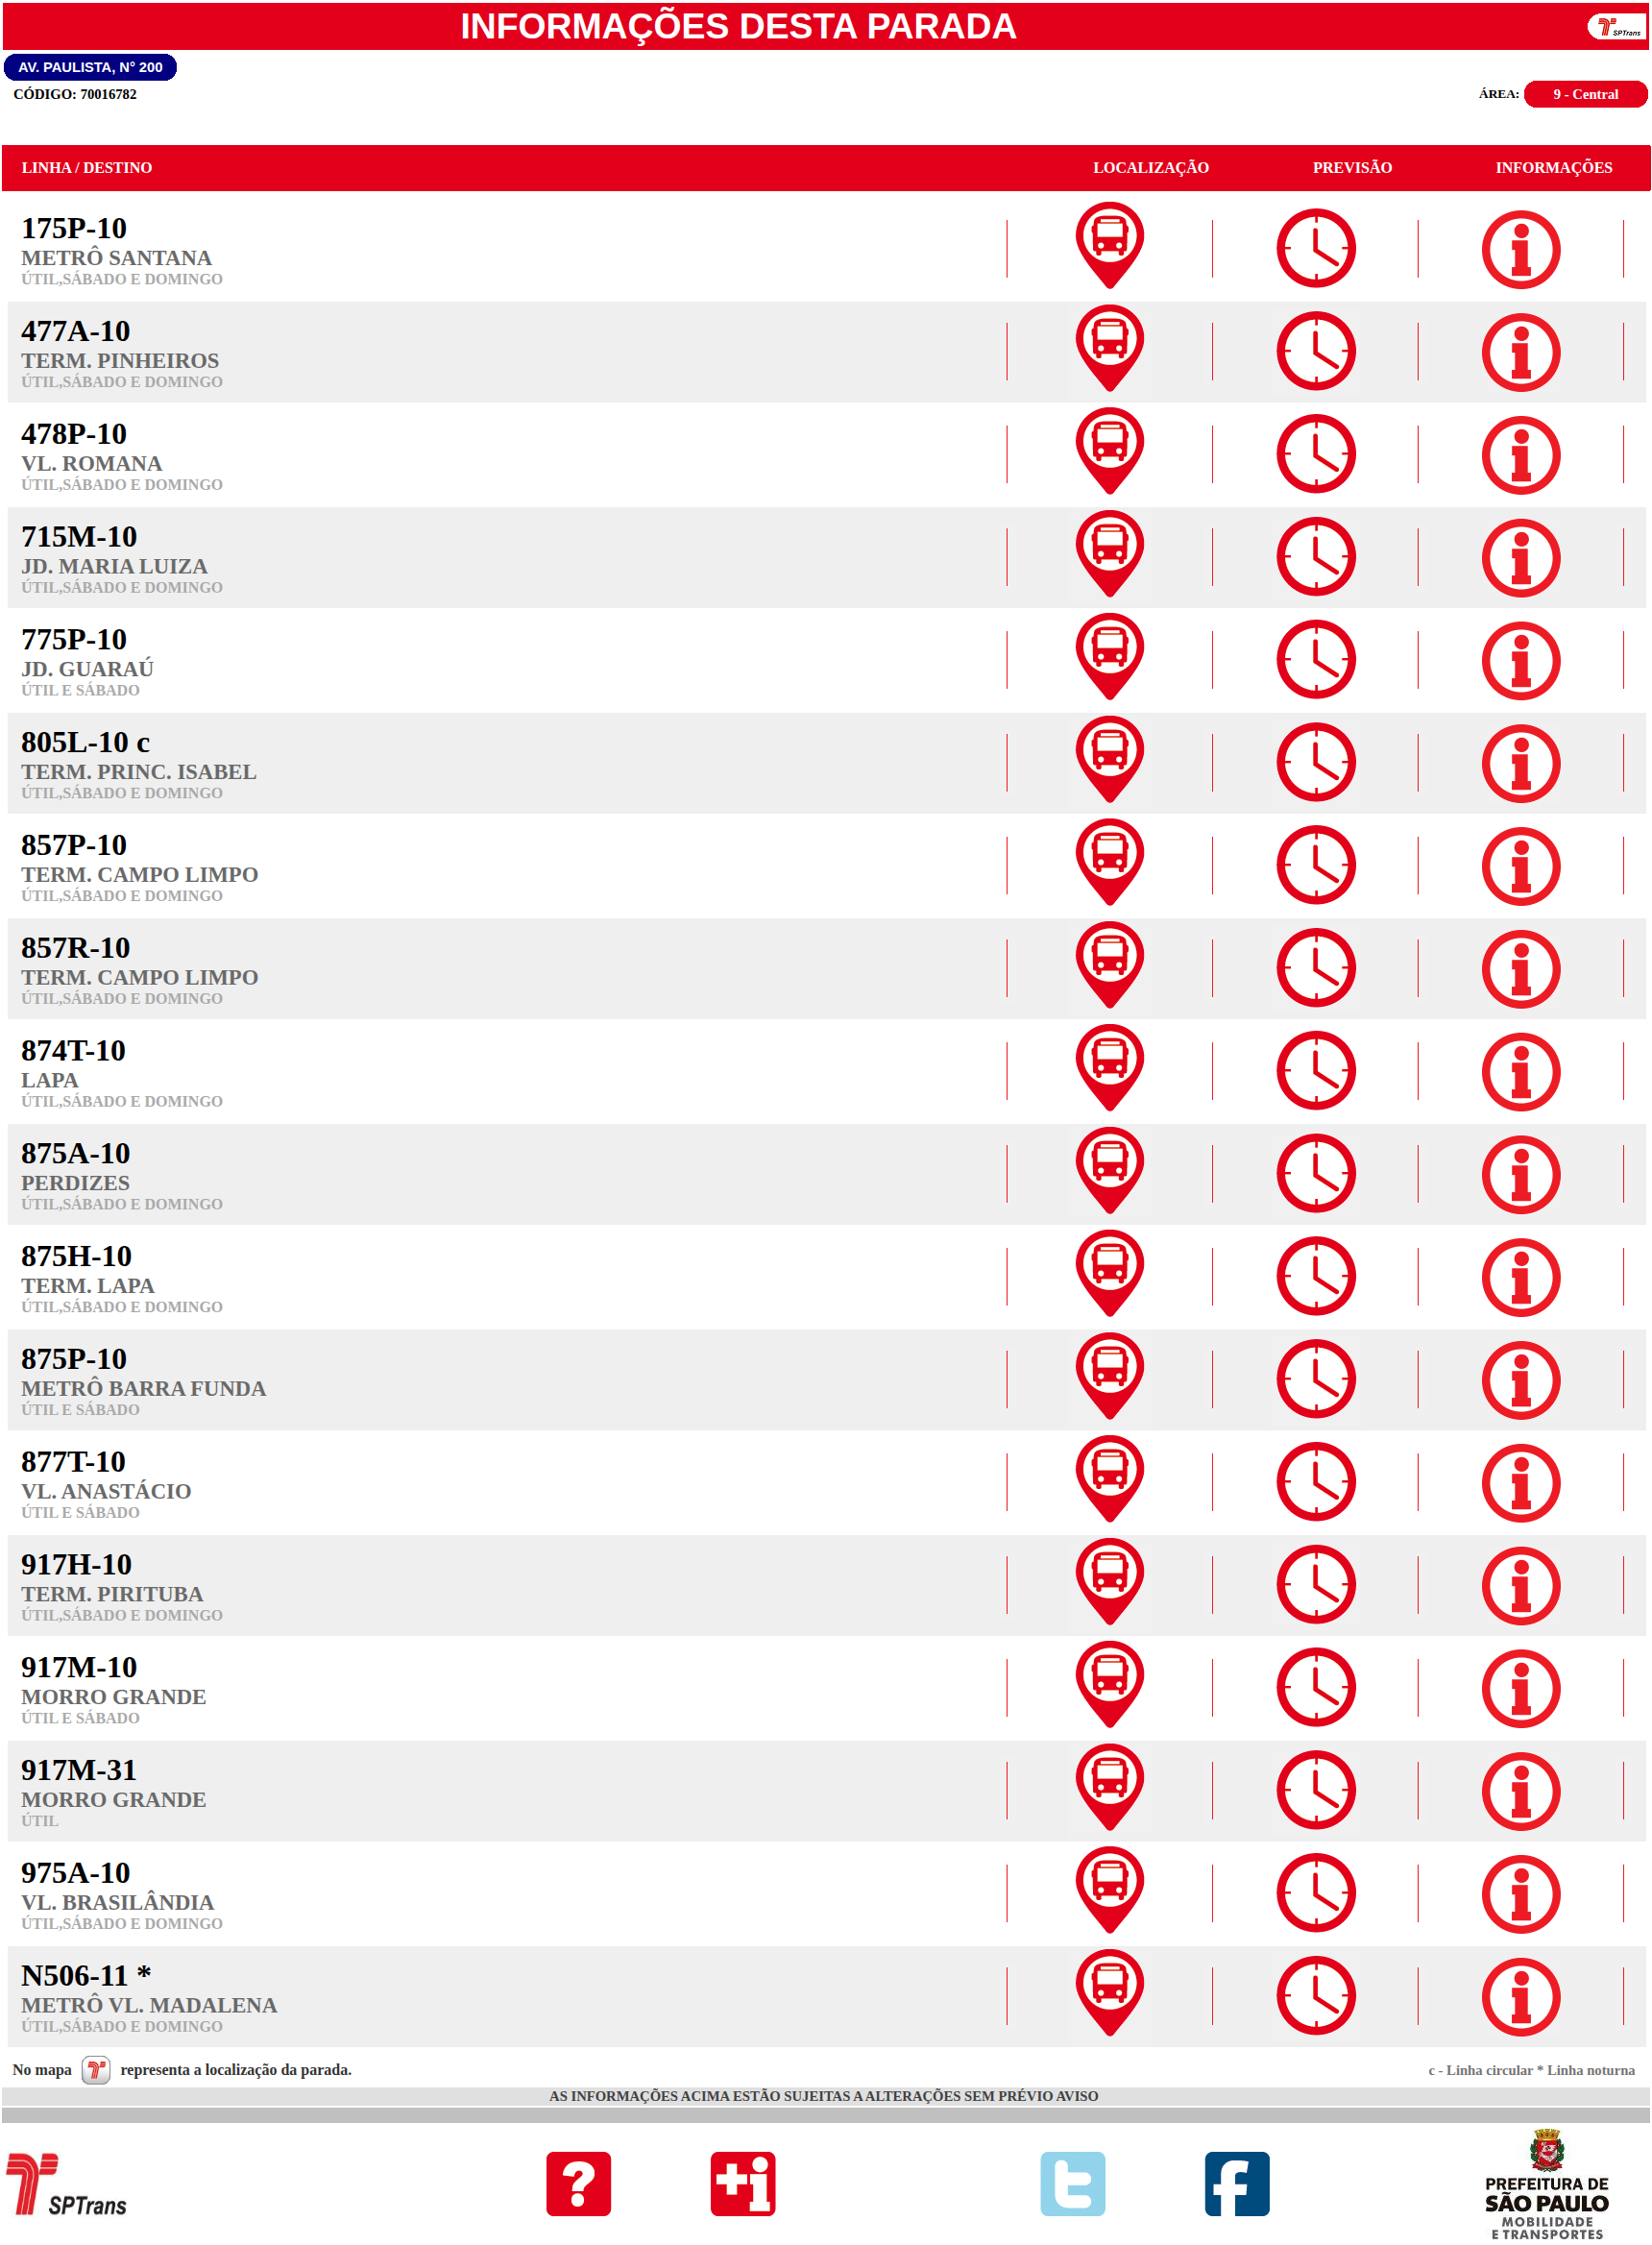
\includegraphics[width=0.95\textwidth,height=0.46\textheight,keepaspectratio]{qrcodeadesivo.extapps.sptrans.com.br-QRCodeAdesivo-adesivo.png}
    \caption{QRCodeAdesivo: ponto identificado pelo QR Code e opções de consulta organizadas por linha.}
    \label{fig:sptrans-parada}
    \fonte{SPTrans, captura de tela fornecida pelo grupo \cite{sptransparada70016782}.}
\end{figure}

\clearpage
\textbf{QRCodeAdesivo: hipótese de descontinuidade da evolução da interface.}
Na verificação técnica de 23 de setembro de 2026, os cabeçalhos HTTP dos arquivos públicos da aplicação do adesivo informaram as datas de última modificação apresentadas na Tabela~\ref{tab:sptrans-modificacao}. O arquivo de código da página e o de configuração indicaram 3 de junho de 2021, enquanto os estilos e uma biblioteca apresentaram datas de 2014 e 2012, respectivamente \cite{sptransadesivojs,sptransgxcfg,sptranscss,sptransgxgral}.

\begin{table}[H]
    \centering
    \caption{Datas declaradas pelo servidor para arquivos da aplicação do adesivo da SPTrans.}
    \label{tab:sptrans-modificacao}
    \begin{tabular}{lll}
        \hline
        Arquivo & Função & \texttt{Last-Modified} \\
        \hline
        \texttt{adesivo.js} & Código da página & 03/06/2021 \\
        \texttt{gxcfg.js} & Configuração & 03/06/2021 \\
        \texttt{GeneXusXEv2.css} & Estilos da interface & 21/05/2014 \\
        \texttt{gxgral.js} & Biblioteca & 01/03/2012 \\
        \hline
    \end{tabular}
    \fonte{Cabeçalhos HTTP dos recursos públicos consultados em 23 set. 2026.}
\end{table}

Na mesma verificação, a página da parada respondeu por HTTP, mas as tentativas de conexão HTTPS expiraram por tempo limite. Não foi possível obter um certificado para verificar sua validade. Esse resultado descreve a condição observada naquele acesso e não permite afirmar que havia um certificado vencido.

As datas dos recursos e a dificuldade de acesso por HTTPS são indícios exploratórios que motivam a hipótese do grupo de defasagem tecnológica e possível descontinuidade da evolução do QRCodeAdesivo. A página ainda respondeu por HTTP na verificação, de modo que não se afirma encerramento do serviço nem descontinuação oficialmente confirmada. Essa hipótese se restringe ao QRCodeAdesivo; os testes de seu domínio não avaliam a manutenção ou a disponibilidade do Olho Vivo.

As datas de \texttt{Last-Modified} são metadados de arquivos específicos e não um histórico de desenvolvimento. Elas não estabelecem a última atualização do backend ou dos dados do QRCodeAdesivo, e arquivos antigos podem continuar adequados ao seu uso. Também não permitem datar atualizações do Olho Vivo, que constitui outro objeto de análise. A confirmação de redução ou interrupção da manutenção dependeria de histórico de versões, observações repetidas ou informação dos responsáveis pelo sistema. Para o PI, os indícios motivam incluir atualização dos dados, manutenção da interface e clareza das mensagens entre os aspectos de avaliação do protótipo.


\clearpage
\subsection{Olho Vivo: consulta de ônibus e escolha da viagem}
\label{sec:analise-olhovivo}
O Olho Vivo é a solução de consulta de ônibus da SPTrans analisada a seguir. As capturas registram buscas, previsões e mapas de consultas distintas no próprio sistema. Os indícios técnicos discutidos para o QRCodeAdesivo não se aplicam a esta análise.

\textbf{1. No acesso pela busca, o passageiro precisa localizar e reconhecer a parada.}
A opção ``De olho no ponto'' solicita um termo de busca. A Figura~\ref{fig:olho-vivo-consultas} mostra esse acesso e a lista retornada para ``05588-000'', na qual é preciso reconhecer a parada por nome, código ou endereço. A consulta por ``Avenida Paulista 200'' não retornou resultados (Figura~\ref{fig:olho-vivo-buscas}), sem que isso comprove ausência da parada na base. Aqui, o passageiro localiza a origem pela busca do Olho Vivo; o QRCodeAdesivo já a identifica pelo código.

\begin{figure}[H]
    \centering
    \begin{minipage}[t]{0.48\textwidth}
        \vspace{0pt}
        \centering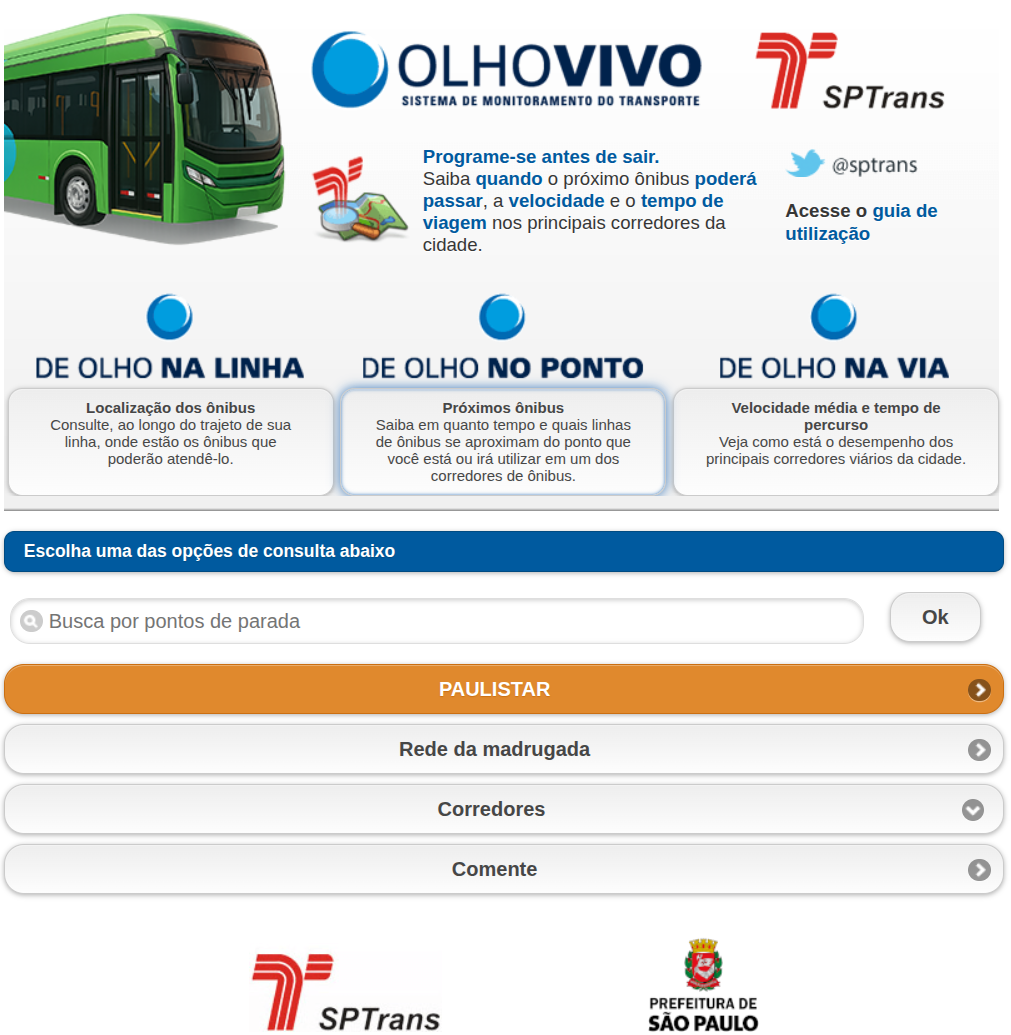
\includegraphics[width=0.86\linewidth]{olho_vivo2.png}
        \par\small (a) Entrada de um termo de busca.
    \end{minipage}\hfill
    \begin{minipage}[t]{0.48\textwidth}
        \vspace{0pt}
        \centering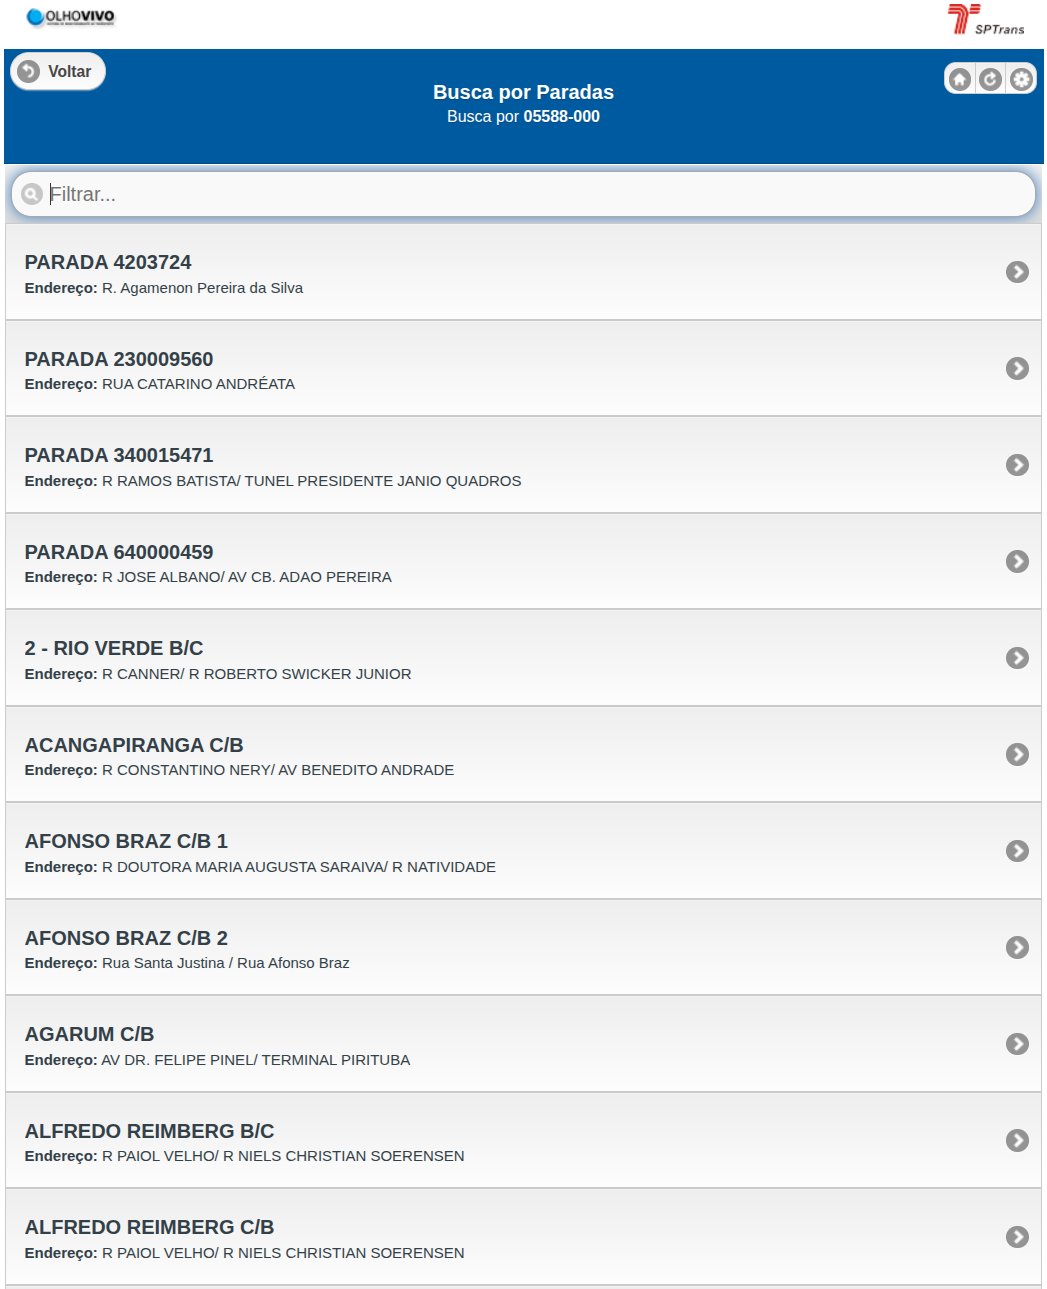
\includegraphics[width=0.86\linewidth]{olho_vivo4.png}
        \par\small (b) Reconhecimento da parada na lista retornada.
    \end{minipage}
    \caption{Olho Vivo, etapa 1: buscar a parada e identificar qual resultado corresponde ao local desejado.}
    \label{fig:olho-vivo-consultas}
    \fonte{SPTrans, sistema Olho Vivo; capturas de tela fornecidas pelo grupo.}
\end{figure}

\begin{figure}[H]
    \centering
    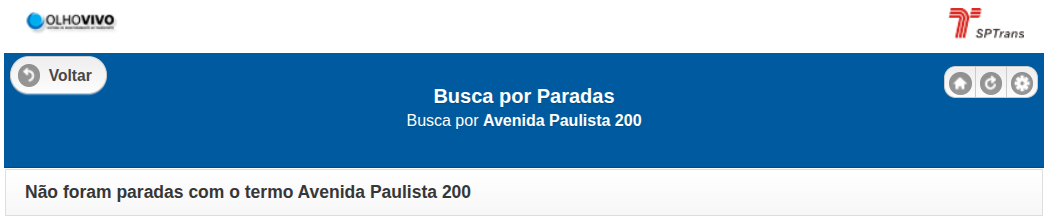
\includegraphics[width=0.95\textwidth]{olho_vivo3.png}
    \caption{Exemplo de busca sem resultados para o termo ``Avenida Paulista 200''.}
    \label{fig:olho-vivo-buscas}
    \fonte{SPTrans, sistema Olho Vivo; captura de tela fornecida pelo grupo.}
\end{figure}

\clearpage
\textbf{2. A consulta do ponto reúne previsões de várias linhas, mas não seleciona as que atendem ao destino.}
A Figura~\ref{fig:olho-vivo-previsoes} mostra as linhas 709M-10, 709A-10 e 709P-10 com previsões de chegada na mesma tela. Portanto, o Olho Vivo já permite acompanhar os próximos ônibus de diferentes linhas na consulta por parada. Essa captura não identifica de forma inequívoca o ponto consultado, que não deve ser presumido como a parada da Avenida Paulista.

\begin{figure}[H]
    \centering
    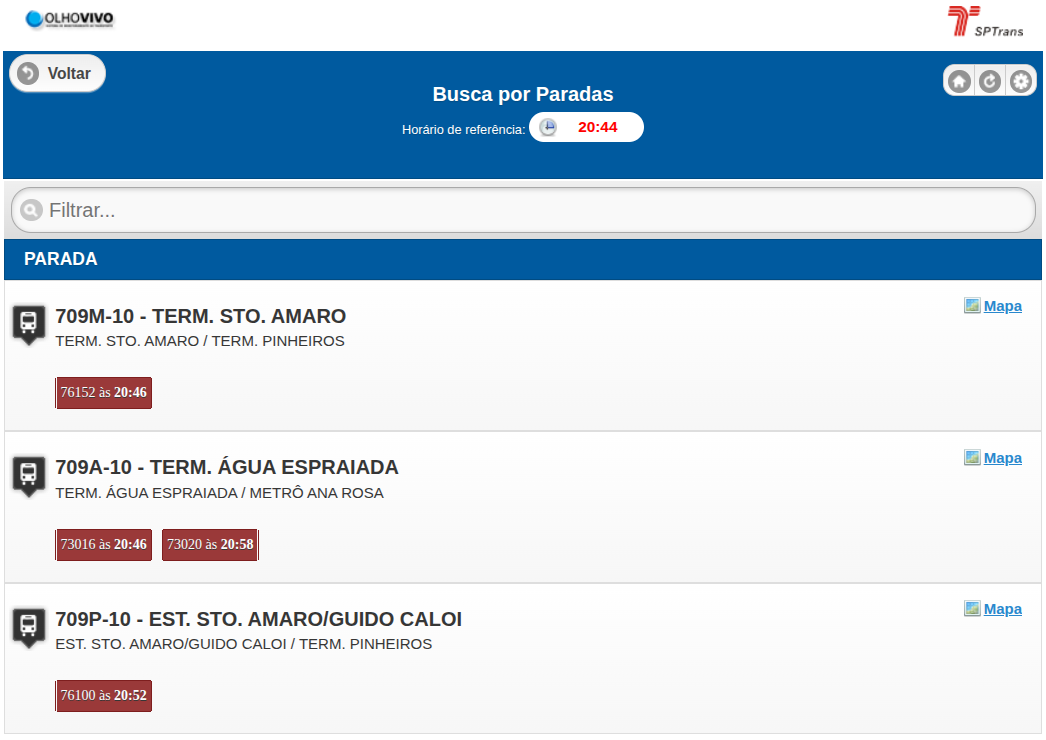
\includegraphics[width=0.95\textwidth]{olho_vivo5.png}
    \caption{Olho Vivo, etapa 2: previsões de várias linhas na mesma tela, com acessos individuais ao mapa.}
    \label{fig:olho-vivo-previsoes}
    \fonte{SPTrans, sistema Olho Vivo; captura de tela fornecida pelo grupo.}
\end{figure}

Saber quais ônibus estão chegando não resolve, por si só, a escolha da viagem. No fluxo registrado, o passageiro precisa conhecer as linhas que atendem ao destino ou investigar seus trajetos. O nome do destino final de uma linha não esclarece necessariamente se ela passa pelo local intermediário desejado. A lista apresenta a oferta do ponto, mas transfere ao usuário a tarefa de reconhecer quais alternativas são úteis para seu deslocamento.

\clearpage
\textbf{3. Uma lista extensa aumenta a informação que precisa ser examinada.}
A captura (Figura~\ref{fig:olho-vivo-lista-extensa}) mostra uma consulta com numerosas linhas e previsões. Para preservar a legibilidade, a imagem foi dividida em dois recortes consecutivos, lidos da esquerda para a direita. O aviso de cookies foi mantido como aparece no registro original.

\begin{figure}[H]
    \centering
    \begin{minipage}[t]{0.48\textwidth}
        \vspace{0pt}
        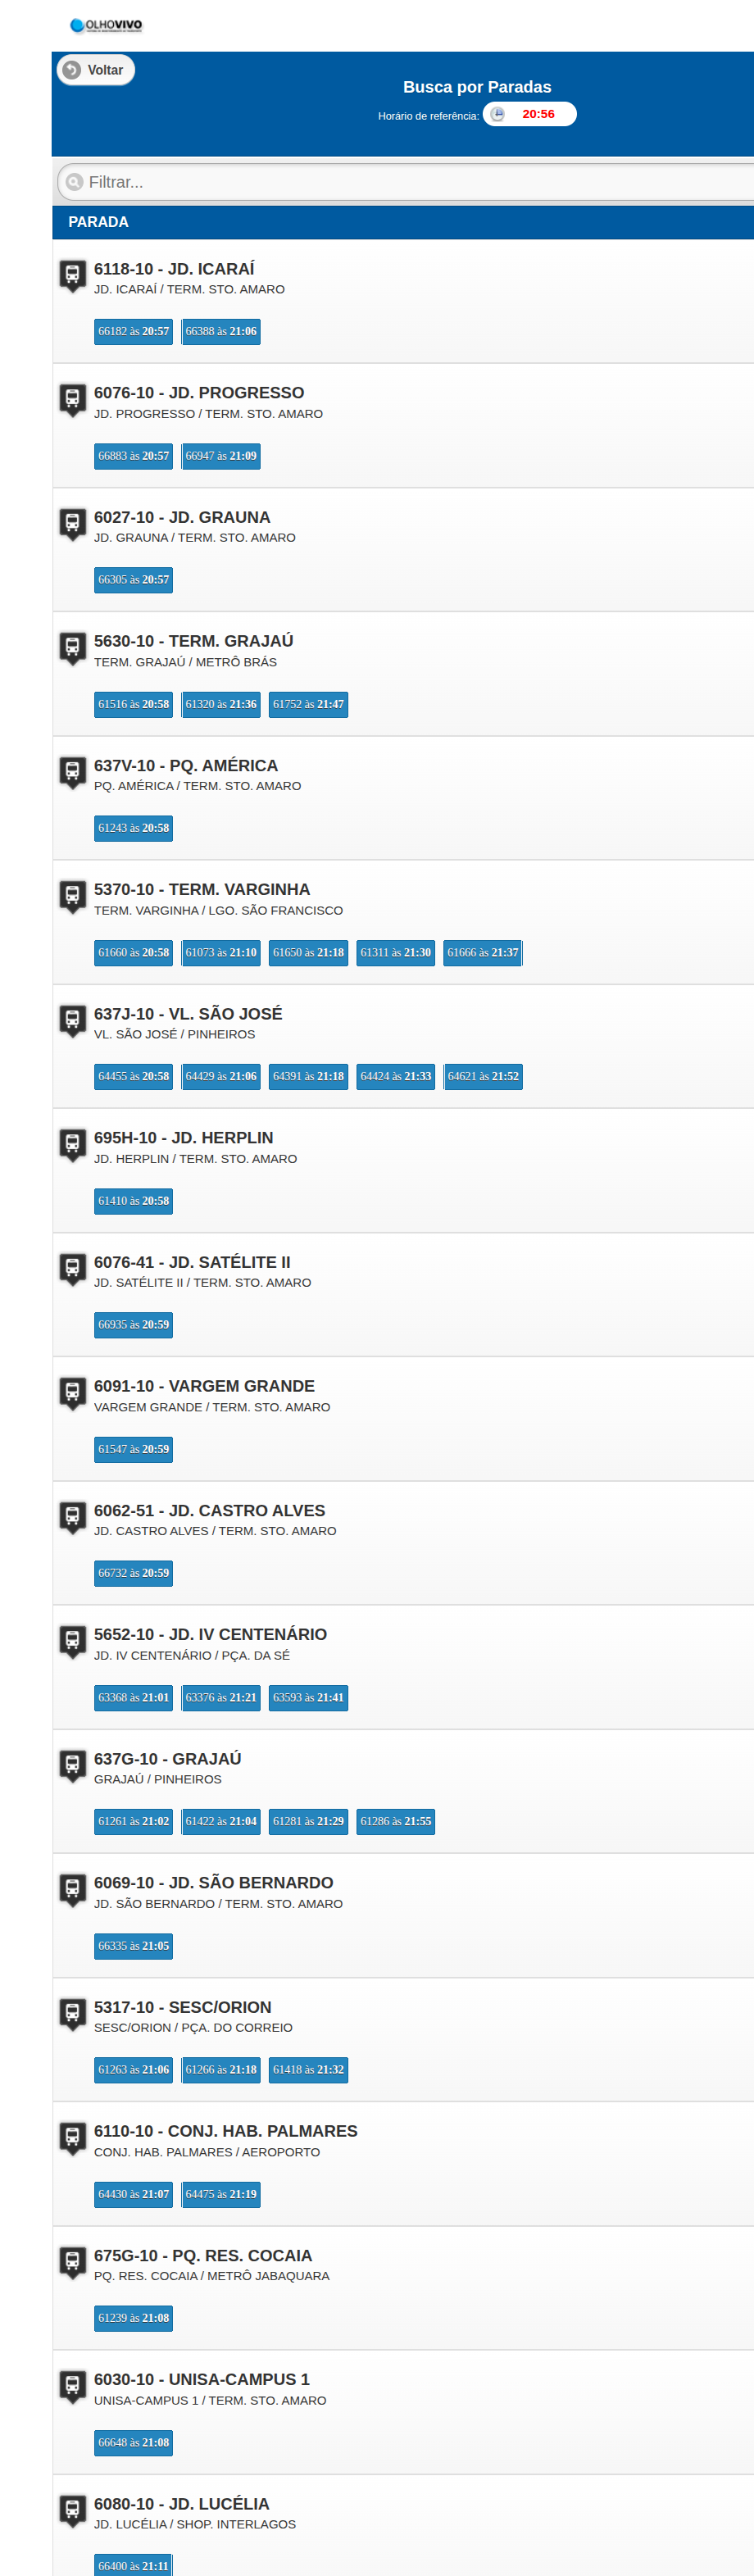
\includegraphics[width=\linewidth,trim=0 1543bp 0 0,clip]{olho_vivo7.png}
        \par\small (a) Parte superior da captura.
    \end{minipage}\hfill
    \begin{minipage}[t]{0.48\textwidth}
        \vspace{0pt}
        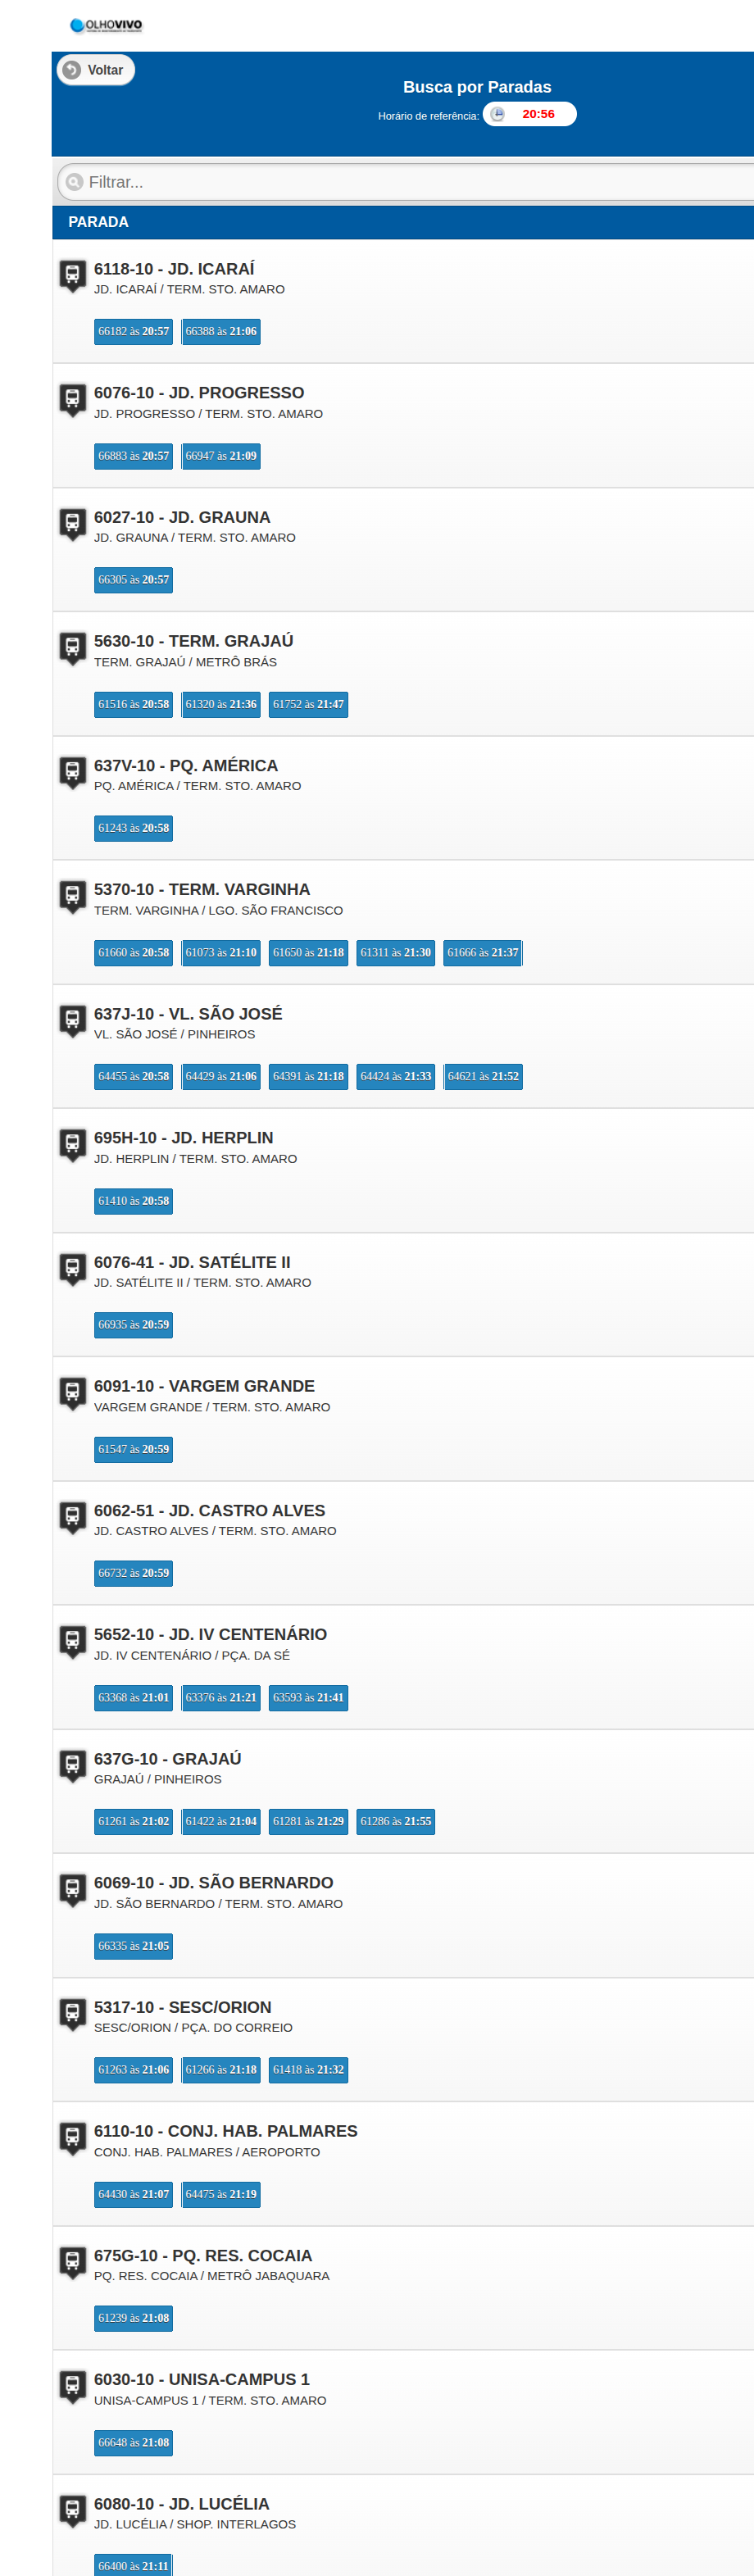
\includegraphics[width=\linewidth,trim=0 0 0 1600bp,clip]{olho_vivo7.png}
        \par\small (b) Continuação da mesma captura.
    \end{minipage}
    \caption{Olho Vivo, etapa 3: lista extensa de linhas e previsões, com informação disponível que ainda precisa ser selecionada conforme o destino do passageiro.}
    \label{fig:olho-vivo-lista-extensa}
    \fonte{SPTrans, sistema Olho Vivo; recortes consecutivos de captura fornecida pelo grupo.}
\end{figure}

A quantidade de opções e a repetição de horários podem gerar sobrecarga visual, sobretudo para quem não conhece a rede. Essa é uma hipótese de usabilidade motivada pelas capturas, a ser avaliada com passageiros. A proposta do PI é reduzir esse esforço mediante a seleção do destino, mantendo visíveis as linhas e conexões relevantes.

\clearpage
\textbf{4. Ao abrir o mapa, o acompanhamento se concentra em uma linha.}
No fluxo observado, o acesso ``Mapa'' de uma linha leva à visualização de seu trajeto e veículos (Figura~\ref{fig:olho-vivo-mapa}). A consulta por ponto reúne linhas em uma lista; o mapa registrado acompanha uma linha por vez. Comparar espacialmente as alternativas exige alternar entre consultas. A captura apresenta o destino ``Est. Sto. Amaro/Guido Caloi'' e o cabeçalho ``LINHA null'', sem permitir confirmar o código da linha apenas pela imagem. Essa inconsistência pertence à tela observada do Olho Vivo e não é usada como evidência de descontinuidade do QRCodeAdesivo.

\begin{figure}[H]
    \centering
    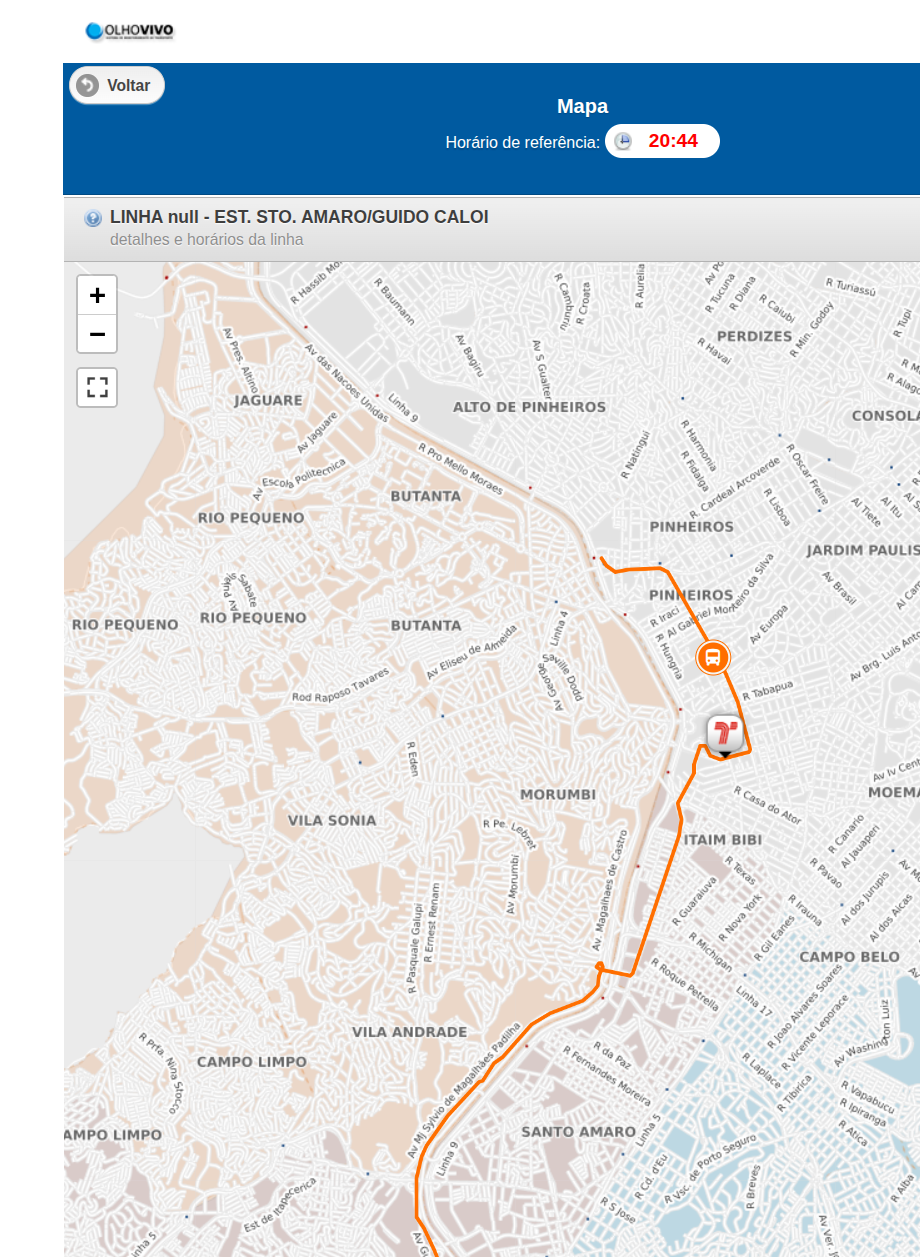
\includegraphics[width=0.95\textwidth,height=0.46\textheight,keepaspectratio]{olho_vivo6.png}
    \caption{Olho Vivo, etapa 4: mapa de um trajeto selecionado, sem visualização conjunta das demais linhas da lista.}
    \label{fig:olho-vivo-mapa}
    \fonte{SPTrans, sistema Olho Vivo; captura de tela fornecida pelo grupo.}
\end{figure}

\textbf{Contribuição pretendida do PI.}
O QRCodeAdesivo é a referência para identificar a origem pelo QR Code; o Olho Vivo é a referência para consultar previsões e veículos. O PI pretende integrar esse acesso ao acompanhamento de diferentes linhas no mesmo mapa e à filtragem por destino, incluindo baldeações. O passageiro informará aonde quer ir, sem precisar conhecer previamente a linha. A utilidade desse fluxo deverá ser validada com a comunidade externa.


\clearpage
\subsection{OpenStreetMap e Overpass API}
O OpenStreetMap é uma base aberta sob ODbL \cite{osmlicense}. Sua modelagem distingue, entre outros elementos, \texttt{stop\_position} e \texttt{platform} \cite{osmpt}. A Overpass API permite consultar elementos por localização, tipo, tags e proximidade \cite{overpass}. O protótipo utiliza Leaflet para a visualização do mapa e das geometrias armazenadas.

\subsection{Geolocalização e responsividade}
A Geolocation API permite solicitar a posição do dispositivo mediante autorização \cite{geolocation}. Como o uso ocorrerá principalmente em smartphones, a interface deverá seguir princípios de Responsive Web Design \cite{responsive}.

\subsection{React no frontend}
React é uma biblioteca JavaScript para construção de interfaces por componentes reutilizáveis \cite{react}. Mapa, ponto selecionado, lista de linhas, trajeto e busca de destino podem ser componentes independentes.

\subsection{Django/Python no backend}
Django é um framework web em Python que oferece uma camada de modelos e ORM para acesso ao banco \cite{django}. No ponto-a-ponto, o backend concentra regras de negócio, persistência, importações e respostas à interface React.

\subsection{Banco de dados}
A implementação utiliza SQLite, no arquivo \texttt{db.sqlite3}, acessado pelo ORM do Django. O banco guarda paradas, linhas, sequências, documentos de origem, estimativas de localização e controles da simulação. Os dados apresentados na aplicação são montados a partir desses registros. PostgreSQL/PostGIS poderá ser considerado se a implantação exigir consultas espaciais ou concorrência mais complexas, mas não compõe a arquitetura atual \cite{postgis}.

\subsection{APIs e integração de dados}
A aplicação importa OSM/Overpass e documentos públicos de catálogos complementares, com normalização antes da gravação no SQLite. Documentos históricos e páginas de conferência não são automaticamente tratados como cadastro operacional. GTFS e APIs de localização continuam como possibilidades de integração, sem fornecimento operacional confirmado para Mauá. A API Olho Vivo é uma referência técnica de dados e endpoints, não a fonte dos veículos simulados do ponto-a-ponto \cite{sptransapi}.

\subsection{Clareza da informação e familiaridade do passageiro}
O documento de Haylett é uma tese de doutorado em Engenharia, apresentada à University of Southampton em 2018. A autora investiga como a familiaridade com o ambiente e com a operação do transporte interfere nas necessidades de informação. Seu quadro \textit{Traveller Planning Types} articula familiaridade e etapas da viagem, e a investigação de planejadores examina a compreensão e a confiança ao planejar deslocamentos conhecidos e desconhecidos \cite{haylett2018}. O PI adapta essas contribuições ao acesso pelo ponto de ônibus; os estudos da tese, especialmente de planejamento prévio no contexto britânico, não demonstram por si só a eficácia do protótipo em Mauá.

Haylett recomenda separar a visão geral das opções dos detalhes necessários para realizar a viagem, apresentar o percurso geográfico e tornar compreensíveis disponibilidade, sentido e complexidade das conexões (p.~138--144). Isso fundamenta um fluxo em que o passageiro reconhece a origem, indica o destino, compara alternativas e então consulta embarque, baldeações e desembarque. A menor duração deve ser apresentada junto às trocas: o caminho mais rápido não é necessariamente o mais simples para quem desconhece a rede \cite{haylett2018}.

A tese também recomenda recuperar consultas sem perda de contexto, evitar resultados antigos após mudanças de destino e explicitar a origem das notificações (p.~144--152). Recomenda agrupar partidas de um mesmo serviço e sentido, preservando diferenças entre trajetos, e reduzir informações periféricas (p.~152--156). No ponto-a-ponto, essas orientações justificam mostrar próximas partidas sem repetir desnecessariamente opções, manter a seleção coerente entre lista e mapa e distinguir dados simulados, posições aproximadas e indisponibilidade de informação \cite{haylett2018}.

\textbf{Requisitos de escopo derivados da leitura.} A revisão estabelece como critérios de evolução e avaliação: consulta inicial sem identificação manual da linha; resumo do deslocamento antes dos detalhes; indicação textual do sentido e das trocas, além das cores do mapa; agrupamento sem misturar variantes ou sentidos; manutenção de origem e destino ao alternar visualizações; e mensagens que distingam falha de consulta, cobertura incompleta e ausência de conexão no cenário. Esses critérios não significam que todos já estejam integralmente atendidos pela interface. Sua verificação com passageiros é uma entrega da próxima etapa, junto à avaliação dos favoritos opcionais em viagens recorrentes.

\subsection{Git e GitHub}
Git é um sistema distribuído de controle de versão, com histórico completo nos clones e suporte a branches para desenvolvimento paralelo \cite{git}.

\section{Metodologia}
A metodologia articula as etapas de ouvir e interpretar o contexto, criar e prototipar, implementar e testar. A revisão da tese de Haylett acrescenta critérios de clareza da informação e um protocolo de avaliação por tarefas. Mantêm-se separados os registros de implementação e as evidências de uso pela comunidade.

\subsection{Ouvir e interpretar o contexto}
Na conversa inicial relatada pelo grupo, Osmar, profissional com passagem pela EMTU, demonstrou interesse pelo acesso às informações por QR Codes nos pontos. Esse contato orientou a proposta, mas não constitui teste de usabilidade nem autorização de implantação. Data, participantes e registro detalhado da conversa ainda precisam ser consolidados. A alegação de ausência da tecnologia em Mauá permanece uma observação do grupo, sem levantamento exaustivo de todos os pontos.

\subsection{Criar e prototipar}
Foram produzidos mockups conceituais e implementado o ponto-a-ponto com Django, React, Leaflet e SQLite. O fluxo associa o QR Code à origem, apresenta alternativas e permite escolher o destino e consultar um percurso. As imagens geradas automaticamente documentam a intenção de interface, enquanto o código e os testes documentam a implementação. Favoritos locais apoiam consultas recorrentes; não se desenvolve aplicativo Android nesta etapa.

A preparação dos dados compreende coleta e preservação das fontes, normalização de identificadores e sequências, importação no banco e geolocalização aproximada dos registros sem coordenadas. Fonte, data, evidências e pendências são mantidas para revisão. Os horários e veículos do cenário de demonstração são separados do cadastro público. A administração controla ativação, relógio e velocidade da simulação; a interface do passageiro informa a natureza demonstrativa dos dados.


\subsection{Coleta, conversão e persistência dos dados}
\label{sec:conversao}
A Tabela~\ref{tab:fontes-publicas} identifica as fontes e sua participação na importação. Os endereços são os utilizados nas coletas registradas pelo projeto, e não uma certificação de disponibilidade ou vigência posterior. O levantamento de transporte do OSM data de 23 de setembro de 2026; a consolidação dos catálogos e a coleta viária foram registradas em 24 de setembro. A data de acesso, a data declarada pelo documento e a data-base da resposta são preservadas separadamente quando disponíveis. Os parâmetros da conversão geográfica e as instruções de reprodução constam do Apêndice~\ref{ap:importacao}.

\begingroup
\small
\setlength{\tabcolsep}{4pt}
\setlength{\parskip}{0pt}
\renewcommand{\arraystretch}{1.15}
\begin{longtable}{>{\raggedright\arraybackslash}p{0.43\textwidth}>{\raggedright\arraybackslash}p{0.52\textwidth}}
\caption{Fontes públicas, endereços de coleta e utilização no ponto-a-ponto}\label{tab:fontes-publicas}\\
\hline
Fonte e endereço & Dados aproveitados e limites \\
\hline
\endfirsthead
\multicolumn{2}{l}{\small Tabela \thetable{} -- continuação}\\
\hline Fonte e endereço & Dados aproveitados e limites \\
\hline
\endhead
\hline \multicolumn{2}{r}{\small Continua na próxima página}\\
\endfoot
\hline
\multicolumn{2}{p{0.95\textwidth}}{\footnotesize Fonte: manifesto, arquivos coletados e scripts de importação do ponto-a-ponto (2026).}\\
\endlastfoot
Cittamobi/Suzantur Mauá\newline
\url{https://linhas.cittamobi.com.br/linhas/estado/sao-paulo/maua/suzantur-maua}
& HTML paginado e páginas de variantes: código, nome, ID, endereço e ordem das paradas; JSON de horários embutido. Foram importadas 164 variantes. Os horários são preservados como metadados, sem conversão automática em viagens operacionais; o HTML coletado não fornece coordenadas numéricas.\\
\hline
PDF Cittamobi, variante 088 Zaira\newline
\url{https://linhas.cittamobi.com.br/maps/transporte_publico-Maua-Suzantur-Maua-088-ZAIRA-169f6fbfd86b.pdf}
& Itinerário, endereços e horários em documento de exemplo, com data declarada de 04/04/2026. Preservação do PDF e extração textual; não substitui as sequências estruturadas nem representa toda a rede.\\
\hline
Suzantur Mauá\newline
\url{https://suzanturmaua.com.br/linhas/}
& Catálogo HTML, páginas individuais e PDFs encontrados: 51 registros de linhas. Código e nome são estruturados; o restante é preservado documentalmente. Não se inventam paradas a partir de listas de ruas.\\
\hline
Prefeitura de Mauá\newline
\url{https://www.maua.sp.gov.br/Noticias/Ler/173}
& Notícia com alterações das linhas 71, 75 e 76: código, nome, itinerário textual por sentido e vigência indicada de 28/02/2026. Três registros incompletos para planejamento, sem coordenadas de embarque.\\
\hline
EMTU: portal e consulta por logradouro\newline
\url{https://www.emtu.sp.gov.br/emtu/itinerarios-e-tarifas.fss}\newline
\url{https://www.emtu.sp.gov.br/Sistemas/linha/resultado.htm?chviatrans=151066&pag=buscarua.htm}
& Tabela HTML de resultado e páginas individuais: seis códigos e nomes, com documentos de itinerários. Consulta parcial; não corresponde ao cadastro integral das linhas intermunicipais de Mauá.\\
\hline
PlanMob, anexo à Lei 5.250/2017\newline
\url{https://sistemas.maua.sp.gov.br/legislaconsulta/atosofic/Leis/5250%20-%20anexo.pdf}
& PDF e texto extraído para diagnóstico histórico e conferência. Propostas, mapas e projeções não se tornam automaticamente linhas vigentes.\\
\hline
Moovit/Suzantur Mauá\newline
\url{https://moovitapp.com/index/pt-br/transporte_p%C3%BAblico-lines-Sao_Paulo-242-3779814}
& Página preservada como documento de conferência. Não houve importação de uma base geográfica completa; a abrangência do catálogo pode ultrapassar o município.\\
\hline
Ônibus Online\newline
\url{https://onibus.online/sp/maua/}
& Página de referência do catálogo, preservada para comparação. Não gera coordenadas ou vínculos de paradas automaticamente.\\
\hline
Bus2 e painel Mobilibus\newline
\url{https://bus2.me/sp/maua/}\newline
\url{https://painel.mobilibus.com/bus2you/home?p=1hl6p}\newline
\url{https://painel.mobilibus.com/public/get-project}
& Páginas de referência e tentativa de consulta POST com \texttt{miniHash=1hl6p}. O endpoint de dados retornou HTTP 500. A falha foi registrada, sem importação de posições ou previsões a partir dessa resposta.\\
\hline
OpenStreetMap/Overpass\newline
\url{https://overpass-api.de/api/interpreter}\newline
\url{https://overpass.kumi.systems/api/interpreter}
& JSON de objetos OSM: 142 registros de paradas/terminais e nove relações no levantamento inicial; recorte separado de ruas e endereços para geolocalização. O segundo servidor foi usado após falha do primeiro na coleta viária. A data-base declarada desse recorte é 15/07/2026.\\
\hline
OSRM: geometria demonstrativa\newline
\url{https://router.project-osrm.org/route/v1/driving}
& Geometrias calculadas para as seis linhas demonstrativas e preservadas localmente. Perfil de automóvel sobre a malha viária, sem homologação como itinerário de ônibus; não fornece localização real dos veículos.\\
\end{longtable}
\endgroup

A transformação das fontes para uso na aplicação ocorre nas seguintes etapas:
\begin{enumerate}
\item \textbf{Coletar e preservar.} O manifesto identifica provedor, URL e tipo de fonte. O coletor percorre a paginação descoberta do Cittamobi e os links de variantes e documentos, mantendo respostas originais, metadados HTTP, data e SHA-256. Uma resposta indisponível ou uma estrutura HTML não reconhecida é registrada como falha, sem preenchimento artificial dos campos ausentes.
\item \textbf{Extrair por formato.} No Cittamobi, o título fornece código e nome; os elementos \texttt{data-stop-id} e os textos dos cartões fornecem identificadores e endereços, preservando a ordem de ocorrência. O bloco JSON \texttt{line-departures-v1} é guardado como metadado de horários. Na Suzantur, são lidos os itens do catálogo; na EMTU, as linhas da tabela de resultado; na notícia municipal, os códigos e os itinerários textuais por sentido. PDFs são convertidos em texto com \texttt{pdftotext -layout}; o HTML documental é limpo sem executar scripts. Extrair texto de um PDF não equivale a transformá-lo automaticamente em rede roteável.
\item \textbf{Normalizar sem perder procedência.} O arquivo \texttt{fonts/collected.json} reúne documentos, paradas e variantes. Identificadores recebem prefixos de fonte, como \texttt{cittamobi:}, e os campos preservam URL, endereço original e atributos complementares. A lista ordenada pode repetir uma parada; fontes diferentes não são unificadas apenas pelo nome ou código. No OSM são preservados tipo, ID e atributos; objetos ferroviários são separados, e o centro de um objeto é tratado como referência geométrica, não como plataforma confirmada.
\item \textbf{Validar e gravar.} A importação verifica hash dos arquivos documentais, identificadores duplicados, existência das paradas referenciadas e pares de coordenadas finitas dentro dos limites geográficos. Quando há durações, exige valores inteiros positivos e quantidade compatível com os segmentos. As rotinas transacionais atualizam registros por ID e recriam a sequência por posição. O Apêndice~\ref{ap:importacao} apresenta o mapeamento dos campos e as regras de reimportação.
\item \textbf{Estimar e auditar coordenadas.} Os endereços sem coordenadas são confrontados com ruas e números OSM. Candidatos são avaliados pela ordem do itinerário e pela conectividade dirigida; decisões e pendências são gravadas por ocorrência e execução. Somente estimativas que atendem aos critérios heurísticos são publicadas, sempre como aproximadas. Essa etapa não valida a existência física da parada.
\item \textbf{Disponibilizar no sistema.} Django consulta o SQLite e fornece os dados à interface React. O catálogo inclui registros incompletos, mas o planejamento exige os atributos necessários ao cenário. As seis linhas demonstrativas entram explicitamente como simuladas. Importar horários documentais ou estimar coordenadas não ativa previsão real nem converte uma variante incompleta em operação válida.
\end{enumerate}

Os mosaicos cartográficos exibidos pelo Leaflet e a busca interativa de endereços por Nominatim são serviços de visualização e consulta separados da importação do cadastro. A geocodificação em lote utiliza o recorte OSM preservado localmente. A interface exploratória Overpass também não substitui a base persistida usada no catálogo do passageiro.

\subsection{Implementar e testar}
A verificação técnica abrange importação, preservação das sequências, estimativas por endereço, cálculo de trajetos, API, preferências e fluxos da interface. Na etapa registrada do desenvolvimento, foram executados com sucesso 58 testes Django e dez testes JavaScript, além de verificações de navegador para o catálogo e a indicação de posições aproximadas. Esses resultados verificam comportamentos programados, não a precisão das coordenadas ou a utilidade do sistema para passageiros.

O planejamento deve permanecer verificável por cenários de viagem direta, baldeação, conexão perdida, permanência no mesmo veículo e ausência de caminho. A comparação com resultados calculados manualmente e o caso de uma partida posterior com chegada anterior permitem conferir a lógica temporal. Alterações futuras dos dados e do algoritmo exigirão repetição dos casos pertinentes.

\textbf{Protocolo proposto para avaliação com a comunidade.} A demonstração a Osmar deverá preceder uma avaliação exploratória com passageiros que relatem diferentes graus de familiaridade com os trajetos, sem tratar essa familiaridade como característica fixa de cada pessoa. Propõem-se as seguintes tarefas:
\begin{enumerate}
\item iniciar a consulta por QR Code sem receber o nome do ponto ou das linhas e indicar um destino;
\item comparar uma alternativa direta com outra que contenha baldeação e explicar a escolha;
\item identificar linha, sentido, embarque, eventual troca e desembarque no percurso escolhido;
\item alterar o destino e verificar a coerência entre lista, mapa e detalhes, sem reutilizar indevidamente o resultado anterior;
\item interpretar uma posição aproximada e uma previsão indisponível, distinguindo-as de localização validada e ausência de ônibus; e
\item salvar e reutilizar um destino favorito, mantendo clara a escolha de outro destino.
\end{enumerate}

Serão registrados conclusão sem ajuda, tempo por tarefa, erros de interpretação, pedidos de auxílio e compreensão das etapas. Uma breve explicação do percurso pelo participante e uma escala de confiança de 1 a 5 complementarão a observação; essa escala é proposta pelo grupo, não um instrumento validado pela tese. Os resultados serão descritivos, com indicação do número e perfil dos participantes e das limitações da amostra. Confiança elevada não será considerada sucesso quando a interpretação estiver incorreta. A participação deverá ser voluntária e os registros minimizados e apresentados sem identificação pessoal.

A avaliação com Osmar e passageiros ainda não foi realizada. O retorno deverá ser documentado, convertido em requisitos e confrontado com os critérios de Haylett. Não se avaliará precisão de previsão real usando horários simulados. A validação operacional das paradas, dos sentidos e dos itinerários será uma atividade distinta, dependente de cadastro autorizado e conferência pelos responsáveis pelo serviço.

\section{Resultados preliminares: solução inicial}

Os resultados desta etapa incluem o protótipo web funcional, a persistência em SQLite, o catálogo importado de fontes públicas, a estimativa auditável de parte das coordenadas e os cenários de planejamento com dados simulados. O acesso por QR Code, a seleção de origem e destino, a consulta de alternativas e os favoritos no navegador estão implementados. A demonstração e a avaliação com a comunidade ainda precisam ocorrer; os mockups não substituem essa evidência.

A contribuição pretendida reúne acesso contextualizado e escolha por destino. Mantém-se a distinção entre as soluções examinadas da SPTrans: o QRCodeAdesivo oferece uma página de parada com links por linha; o Olho Vivo apresenta, nas capturas analisadas, previsões de várias linhas por ponto e mapa de uma linha selecionada. O ponto-a-ponto busca integrar comparação e filtragem no mesmo fluxo. A análise não estabelece superioridade do protótipo nem limitação de todos os serviços da SPTrans.

\subsection{Base de dados OSM utilizada no desenvolvimento}

O protótipo utiliza o OpenStreetMap como base para o desenvolvimento. Em levantamento realizado pela Overpass API em 23 de setembro de 2026, com base de dados atualizada nessa data e recorte pelo limite municipal de Mauá, foram encontrados 112 objetos de pontos de ônibus, três plataformas adicionais de ônibus, 21 posições de parada dos veículos e seis objetos classificados como terminais. Essas quantidades representam objetos do OSM, e não locais físicos necessariamente distintos: uma parada ou um terminal pode possuir múltiplas representações. Os objetos ferroviários foram separados do inventário de ônibus.

A consulta retornou nove relações de trajetos de ônibus, correspondentes a cinco códigos: 160, 284M, 285, 4028-10 e AL110. O resultado inclui serviços de municípios vizinhos e elementos próximos às divisas; não constitui um inventário completo das linhas municipais. Apenas dois objetos locais de parada aparecem como membros das relações de trajetos retornadas. Na consulta realizada, não foi identificada uma rede de rotas municipais da Suzantur Mauá, embora esse operador conste no cadastro do terminal municipal. A consulta, a resposta original e os inventários foram preservados pelo grupo para permitir a reprodução e a revisão do levantamento.

O levantamento OSM constitui uma das bases do catálogo, complementada por outras fontes públicas. Seus objetos preservam os identificadores de origem; não são fundidos automaticamente com paradas de outro provedor apenas pela semelhança de endereço. A cobertura incompleta não é interpretada como ausência de serviço.

\subsection{Catálogo importado e localização aproximada}
O inventário consolidado em 24 de setembro de 2026 contém 1.616 registros de paradas e terminais: 1.474 do Cittamobi e 142 do OSM. Desses, 172 possuem coordenadas: os 142 registros OSM e 30 estimativas produzidas por endereço e contexto do itinerário. Permanecem 1.444 registros sem coordenadas. Nem a origem OSM nem a aceitação pelo algoritmo equivalem a validação de campo. As contagens representam registros de fontes, não necessariamente locais físicos distintos.

O banco contém 233 registros não demonstrativos de linhas ou variantes, distribuídos conforme a Tabela~\ref{tab:catalogo}. Existem ainda seis linhas fictícias de demonstração, totalizando 239 registros. As fontes se sobrepõem e diferenciam sentidos e variantes; portanto, 233 não é o número de linhas únicas em operação em Mauá.

\begin{table}[htbp]
\centering
\caption{Registros de linhas e variantes por fonte no catálogo importado}
\label{tab:catalogo}
\begin{tabular}{lrr}
\hline
Fonte & Registros & Códigos distintos na fonte \\
\hline
Cittamobi/Suzantur Mauá & 164 & 53 \\
Suzantur Mauá & 51 & 51 \\
EMTU (consulta parcial) & 6 & 6 \\
OpenStreetMap & 9 & 5 \\
Prefeitura de Mauá & 3 & 3 \\
\hline
Total de registros & 233 & --- \\
\hline
\end{tabular}
\fonte{Banco do ponto-a-ponto e registros de importação do grupo, 24 set. 2026.}
\end{table}

O Cittamobi fornece identificadores, endereços e sequências; a Suzantur, catálogos e páginas de linhas. A publicação municipal registra alterações das linhas 71, 75 e 76, enquanto a consulta da EMTU cobre apenas o resultado de um logradouro. PlanMob de 2017, Moovit, Ônibus Online e Bus2 foram preservados como referências ou documentos de conferência. O PlanMob não foi convertido em operação vigente. A consulta de dados do painel Bus2 retornou erro HTTP 500 e não forneceu dados operacionais. As fontes e seus limites estão descritos no manifesto \texttt{fonts/sources.json} e no documento técnico de importações \cite{mbmimportacoes}.

As respostas originais são preservadas em \texttt{fonts/raw/}, com endereço de origem, data de coleta e hash SHA-256; a normalização é registrada antes da importação. O banco relaciona documentos, paradas, linhas e posições na sequência. Uma parada pode aparecer mais de uma vez no mesmo itinerário, sem perda dessa ordem. Reimportações preservam a identidade dos registros por fonte; o desaparecimento de uma página não é tratado automaticamente como encerramento de uma linha.

A geolocalização utiliza a versão \nolinkurl{osm-address-directed-v1.1}, documentada no projeto \cite{mbmimportacoes}. O procedimento normaliza rua e número, procura endereços numerados no recorte OSM e gera candidatos na via. Quando possível, usa o número exato ou interpolação entre endereços conhecidos; não extrapola a numeração. Em seguida, considera conjuntamente os candidatos pela sequência das paradas e pela conectividade de um grafo viário direcionado, respeitando os sentidos e restrições reconhecidos. Nessa etapa auxiliar usa-se busca A* para distâncias viárias; o planejador de viagens continua utilizando Dijkstra.

A escolha exige evidência suficiente e separação entre alternativas ambíguas. Estimativas de um mesmo identificador são conciliadas entre variantes; divergências de posição ou sentido impedem sua publicação como coordenada consensual. Um deslocamento lateral de três metros à direita do sentido inferido é uma hipótese geométrica, não confirmação do lado de embarque ou da calçada. A aplicação identifica as posições estimadas como aproximadas e preserva as evidências para revisão. Nenhuma estimativa é marcada automaticamente como validada.

A execução analisou 3.735 ocorrências de paradas em 164 variantes. Aceitou 272 ocorrências, correspondentes a 30 identificadores distintos após a conciliação; as demais 3.463 ocorrências permaneceram pendentes por rua não localizada ou ambígua, indefinição do endereço/sentido ou falta de caminho direcionado. O recorte viário coletado em 24 de setembro contém 26.393 objetos e declara data-base de 15 de julho de 2026, anterior ao acesso. Essas restrições impedem apresentar as estimativas como cadastro completo ou atualizado da operação municipal.

A inclusão de um registro no mapa não o torna apto ao planejamento. As geometrias das seis linhas demonstrativas foram calculadas sobre ruas por OSRM com perfil viário de automóvel e preservadas no banco; não são itinerários de ônibus homologados. Horários, intervalos, deslocamentos e posições dos veículos continuam simulados. Essa separação permite demonstrar o funcionamento sem atribuir ao OSM ou aos catálogos previsões que eles não forneceram.

\subsection{Fluxo funcional do protótipo demonstrativo}

O fluxo implementado no cenário demonstrativo e preparado para apresentação à comunidade externa é:

\begin{enumerate}
\item o usuário lê o QR Code do ponto e abre a consulta no navegador, sem precisar instalar um aplicativo ou informar previamente linha, ponto ou endereço; alternativamente, acessa diretamente o mapa;
\item o QR Code identifica automaticamente a origem; no acesso direto ao mapa, o usuário seleciona uma parada;
\item o sistema recupera as linhas associadas ao ponto de origem;
\item o cenário mockado fornece as posições e os horários dos veículos; para cada linha, o sistema exibe o ônibus simulado mais próximo que se desloca em direção ao ponto selecionado, com indicação de simulação na interface;
\item os veículos são representados no mapa e acompanhados de identificação da linha e informação de aproximação;
\item o usuário seleciona um ponto de destino;
\item o sistema aplica Dijkstra para buscar um caminho de menor tempo estimado, considerando horários, sentido das viagens, espera e eventuais baldeações;
\item são destacadas as linhas do caminho encontrado, inclusive as conexões posteriores, e ocultadas as demais alternativas;
\item o mapa passa a apresentar somente os trajetos e veículos relevantes;
\item são apresentados o tempo total e o horário estimado de chegada, os trechos de cada linha e os pontos de troca; caso não haja caminho nos dados e na janela consultados, essa limitação é informada ao usuário.
\end{enumerate}

A API Olho Vivo da SPTrans demonstra a viabilidade técnica desse tipo de interação em uma fonte operacional: sua documentação prevê consulta de todas as linhas que atendem uma parada, posição dos veículos e previsão de chegada por parada e linha. Essa API não é assumida como fonte de dados de Mauá; é utilizada como referência técnica para o tipo de dado que uma integração operacional pode fornecer.

\clearpage
\subsection{Mockups gerados automaticamente: sequência de uso}
As Figuras~\ref{fig:mockup-origem} a~\ref{fig:mockup-detalhes} apresentam oito imagens conceituais geradas automaticamente, organizadas em quatro pares para orientar a implementação e a apresentação a Osmar. Não são capturas de um sistema já implementado. Nomes de linhas, endereços, mapas, horários e tempos são ilustrativos e não comprovam correspondência com a operação de Mauá ou com os registros do OSM. Os elementos de identificação municipal da primeira imagem não representam instalação ou aprovação oficial, e o QR Code desenhado não é apresentado como código funcional.

\textbf{1. Ler o QR Code e reconhecer a origem.}
O primeiro par mostra a sinalização imaginada para o ponto e a interface aberta com a origem identificada. A intenção é dispensar a pesquisa prévia do nome, código ou endereço da parada e oferecer acesso às linhas ou à escolha do destino (Figura~\ref{fig:mockup-origem}).

\begin{figure}[H]
    \centering
    \begin{minipage}[t]{0.48\textwidth}
        \vspace{0pt}\centering
        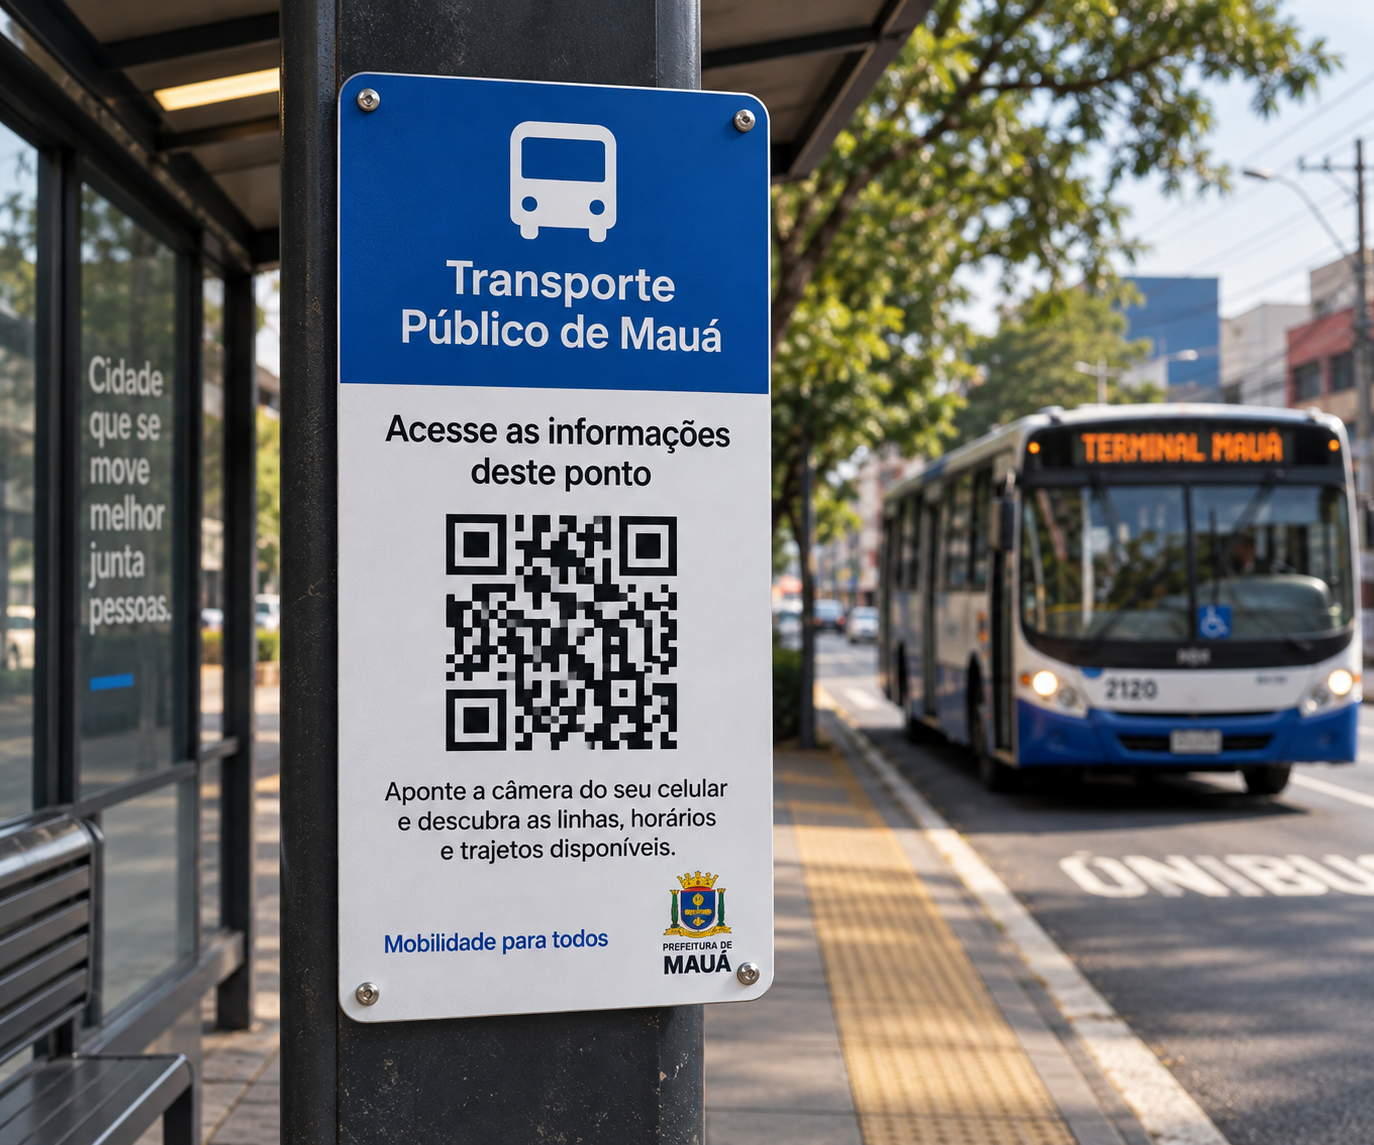
\includegraphics[width=\linewidth,height=0.52\textheight,keepaspectratio]{mockup1.png}
        \par\small (a) Sinalização conceitual com QR Code.
    \end{minipage}\hfill
    \begin{minipage}[t]{0.48\textwidth}
        \vspace{0pt}\centering
        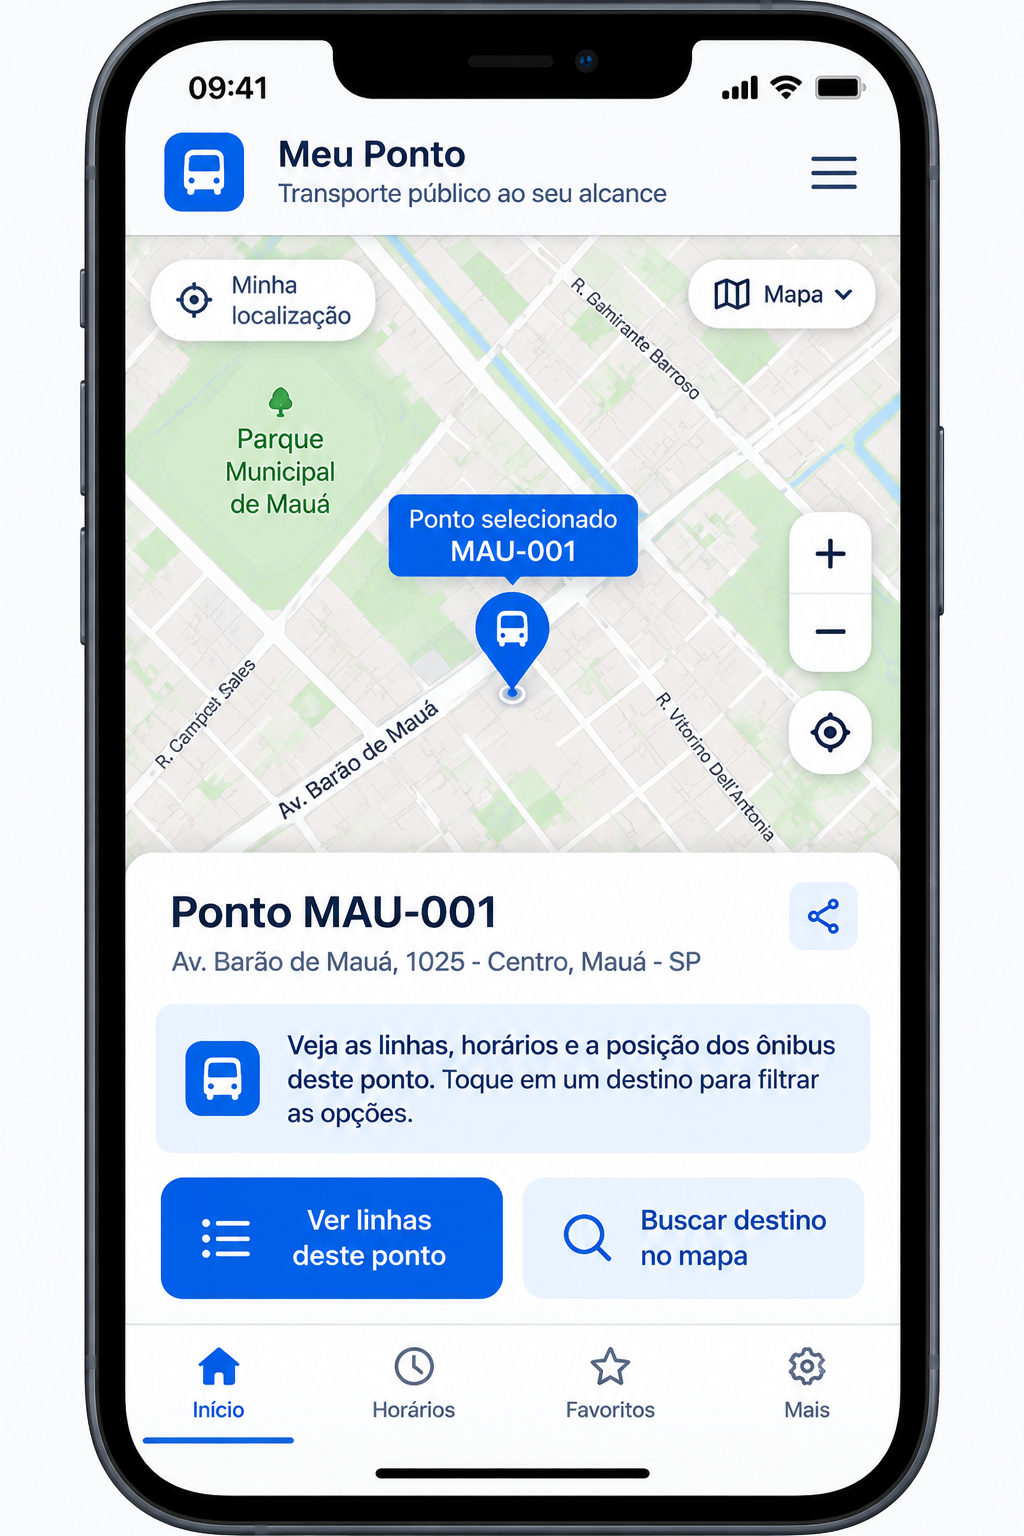
\includegraphics[width=\linewidth,height=0.52\textheight,keepaspectratio]{mockup2.png}
        \par\small (b) Origem identificada na interface.
    \end{minipage}
    \caption{Mockups: acesso no ponto de ônibus e identificação da origem.}
    \label{fig:mockup-origem}
    \fonte{Mockups gerados automaticamente e fornecidos pelo grupo (2026); dados ilustrativos.}
\end{figure}

\clearpage
\textbf{2. Consultar os próximos ônibus e escolher o destino.}
A lista inicial apresenta as linhas do ponto com tempos simulados de aproximação. O passageiro pode selecionar o destino no mapa ou na busca, sem precisar decidir antecipadamente qual linha utilizar (Figura~\ref{fig:mockup-destino}). A lista completa funciona como uma visão inicial; a seleção do destino deverá permitir reduzir as informações às alternativas úteis para a viagem.

\begin{figure}[H]
    \centering
    \begin{minipage}[t]{0.48\textwidth}
        \vspace{0pt}\centering
        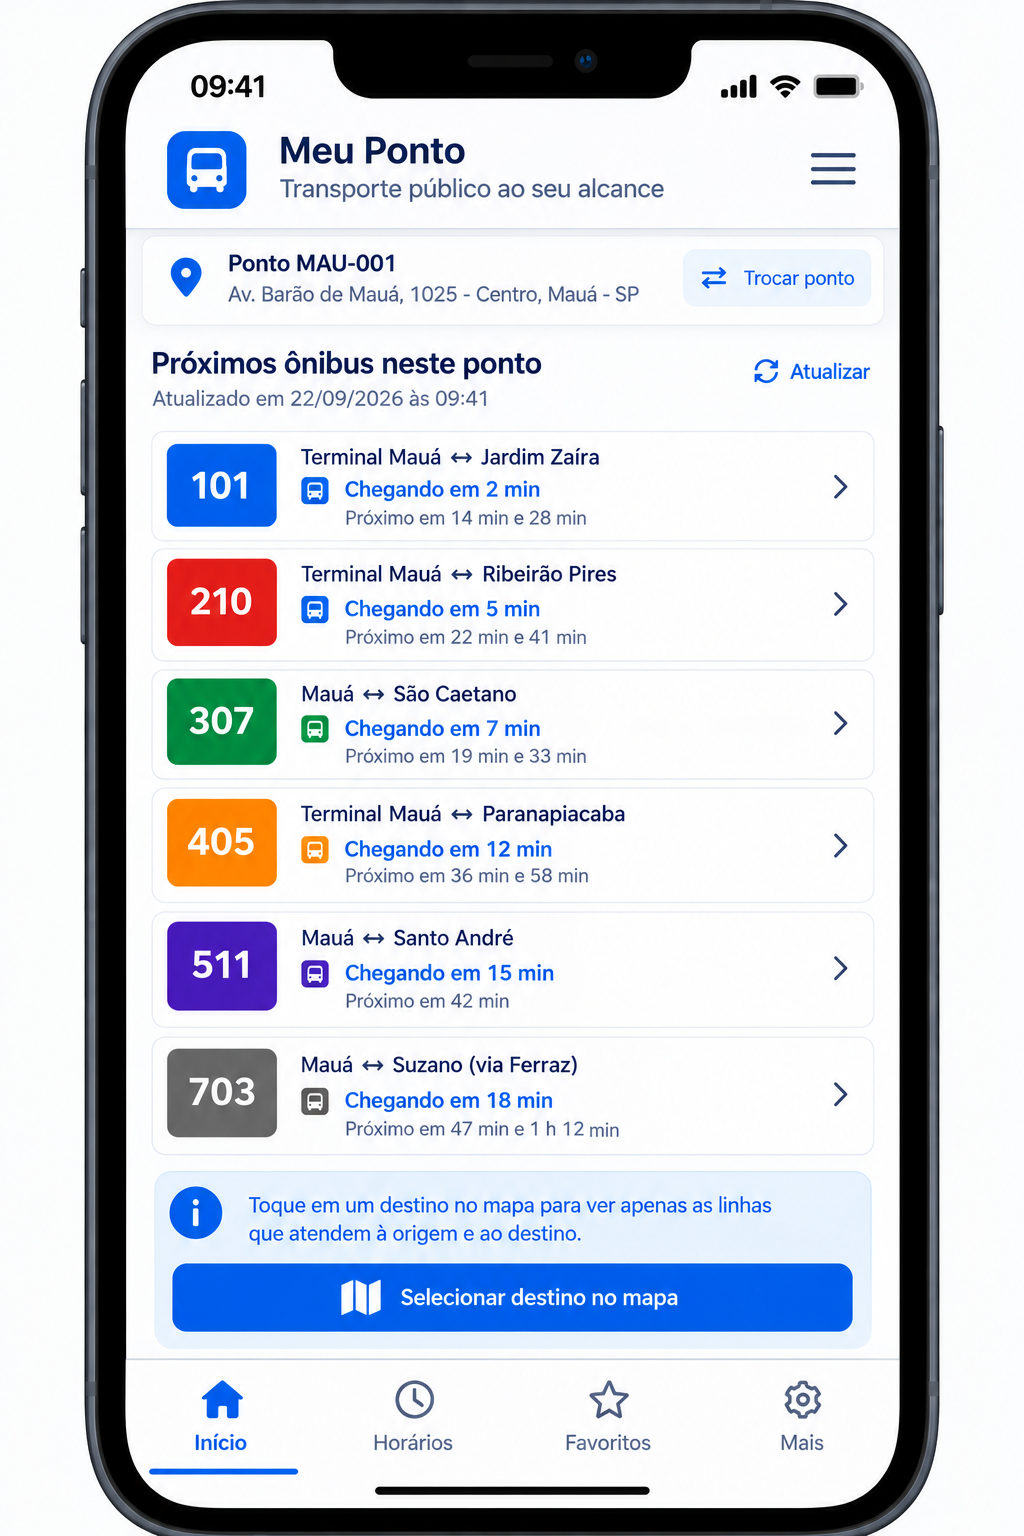
\includegraphics[width=\linewidth,height=0.52\textheight,keepaspectratio]{mockup3.png}
        \par\small (a) Linhas e próximos ônibus do ponto.
    \end{minipage}\hfill
    \begin{minipage}[t]{0.48\textwidth}
        \vspace{0pt}\centering
        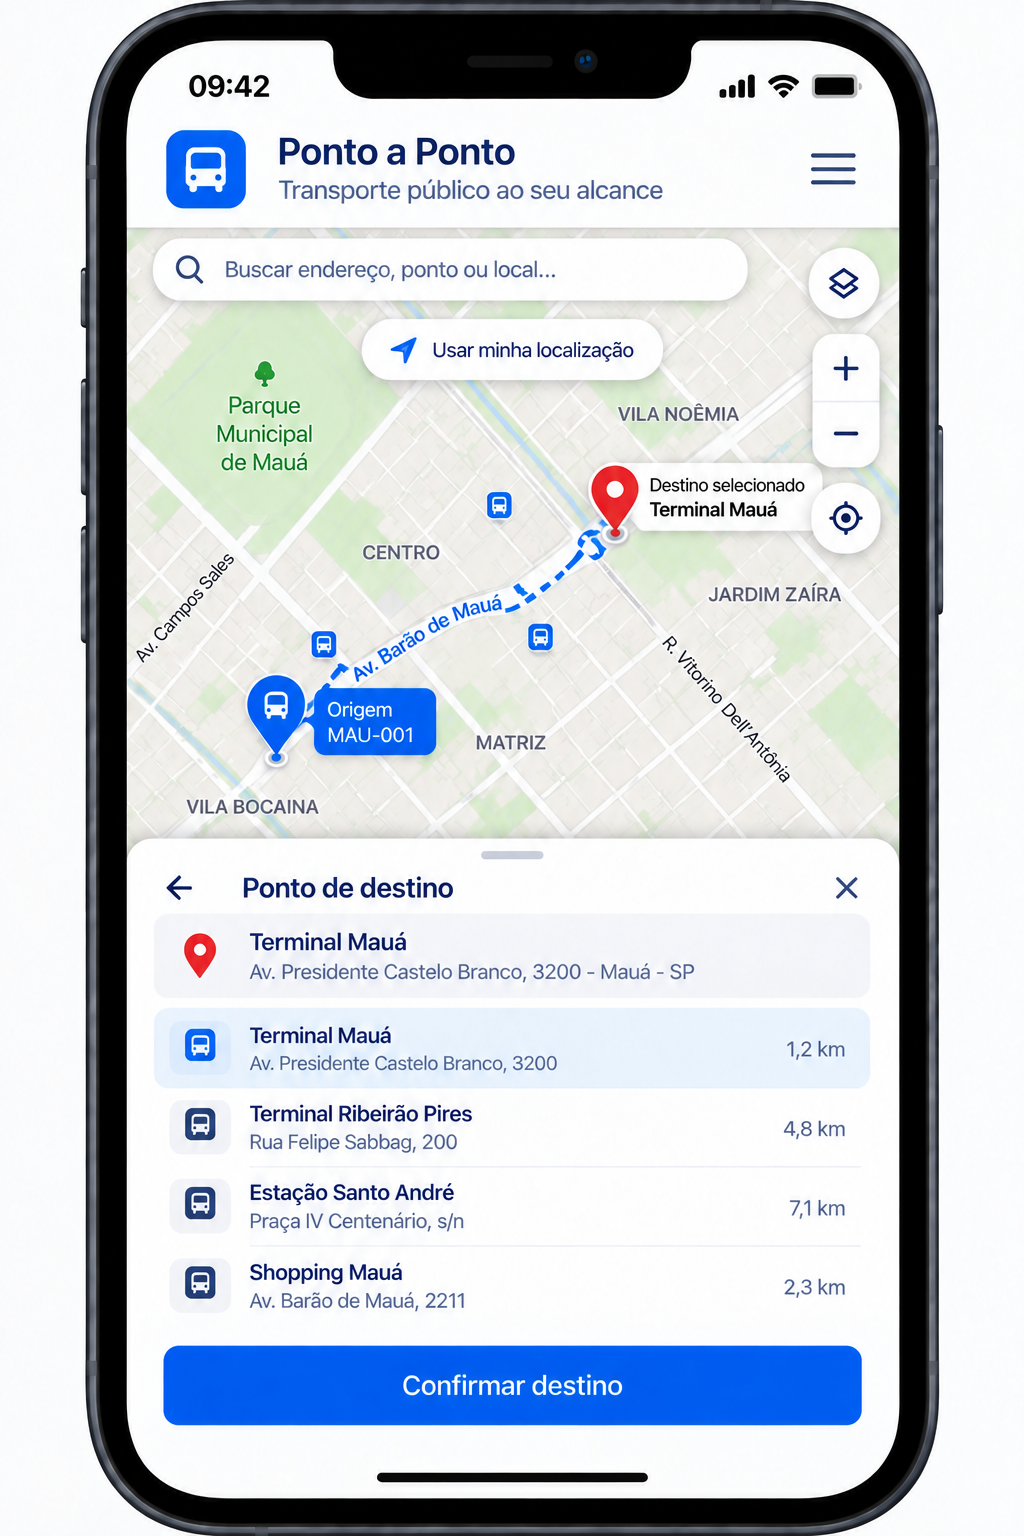
\includegraphics[width=\linewidth,height=0.52\textheight,keepaspectratio]{mockup4.png}
        \par\small (b) Escolha e confirmação do destino.
    \end{minipage}
    \caption{Mockups: consulta inicial das linhas e seleção do destino.}
    \label{fig:mockup-destino}
    \fonte{Mockups gerados automaticamente e fornecidos pelo grupo (2026); dados ilustrativos.}
\end{figure}

\clearpage
\textbf{3. Filtrar as alternativas e acompanhar diferentes linhas no mesmo mapa.}
Após a definição do destino, o par da Figura~\ref{fig:mockup-fluxo} mostra uma lista reduzida e um mapa que reúne veículos de diferentes linhas. As cores ajudam a relacionar cada veículo à respectiva alternativa. Essa etapa ilustra a integração pretendida pelo PI: o passageiro compara os ônibus úteis ao deslocamento, sem alternar entre mapas individuais de cada linha. As posições e os tempos exibidos pertencem ao cenário simulado.

\begin{figure}[H]
    \centering
    \begin{minipage}[t]{0.48\textwidth}
        \vspace{0pt}\centering
        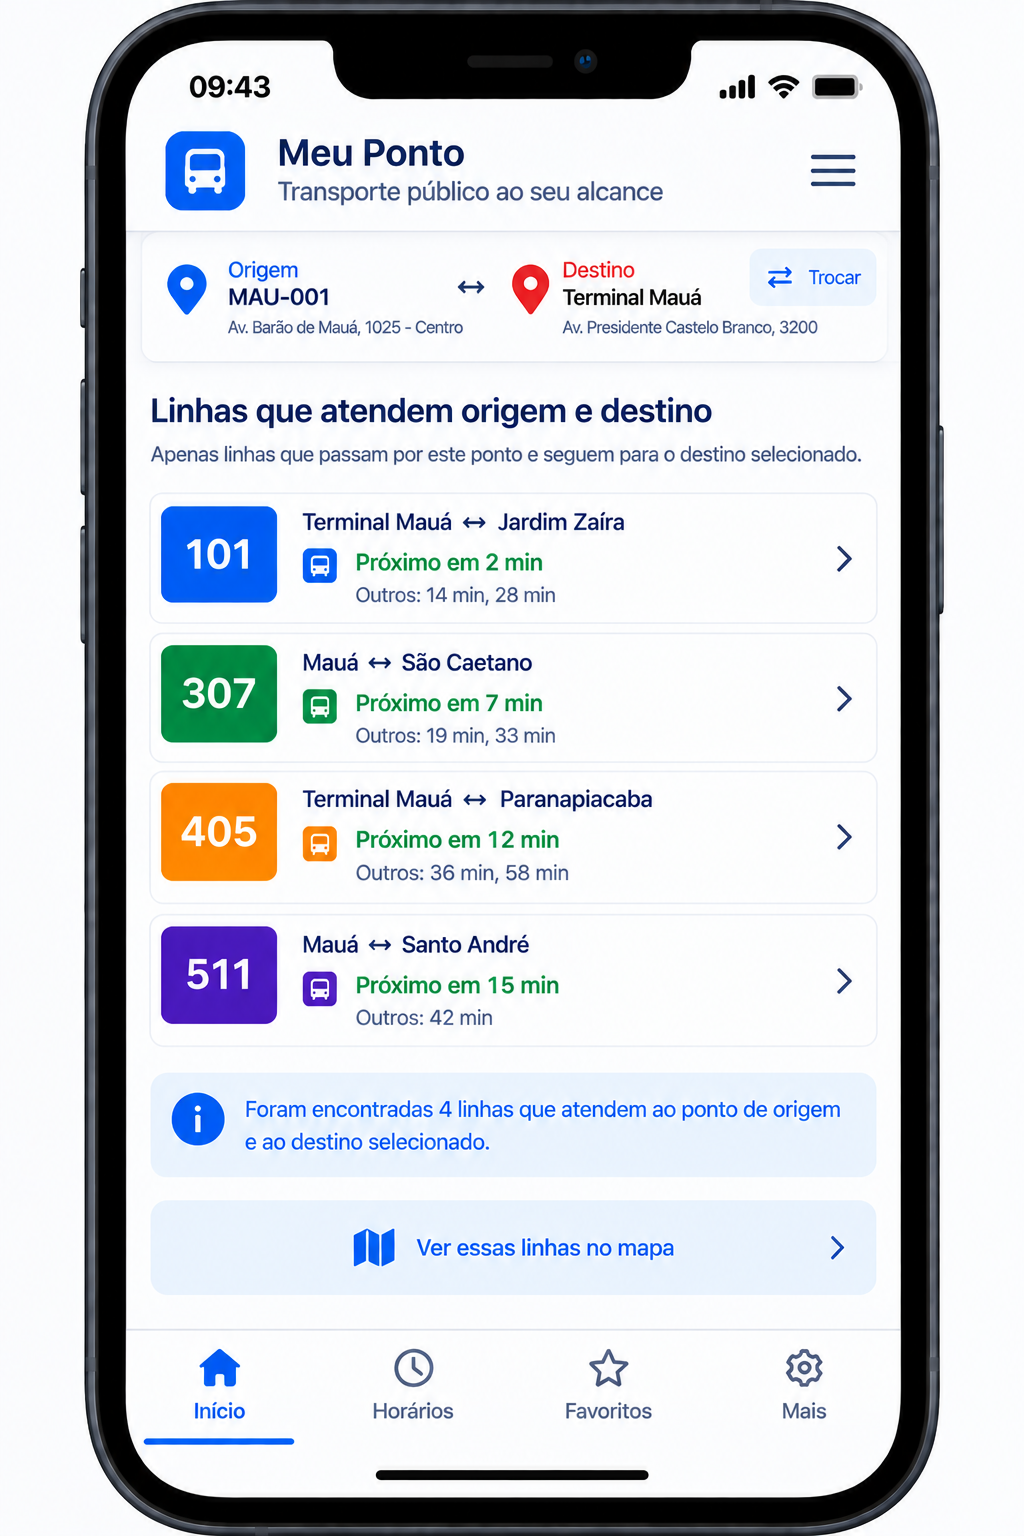
\includegraphics[width=\linewidth,height=0.52\textheight,keepaspectratio]{mockup5.png}
        \par\small (a) Alternativas filtradas pelo destino.
    \end{minipage}\hfill
    \begin{minipage}[t]{0.48\textwidth}
        \vspace{0pt}\centering
        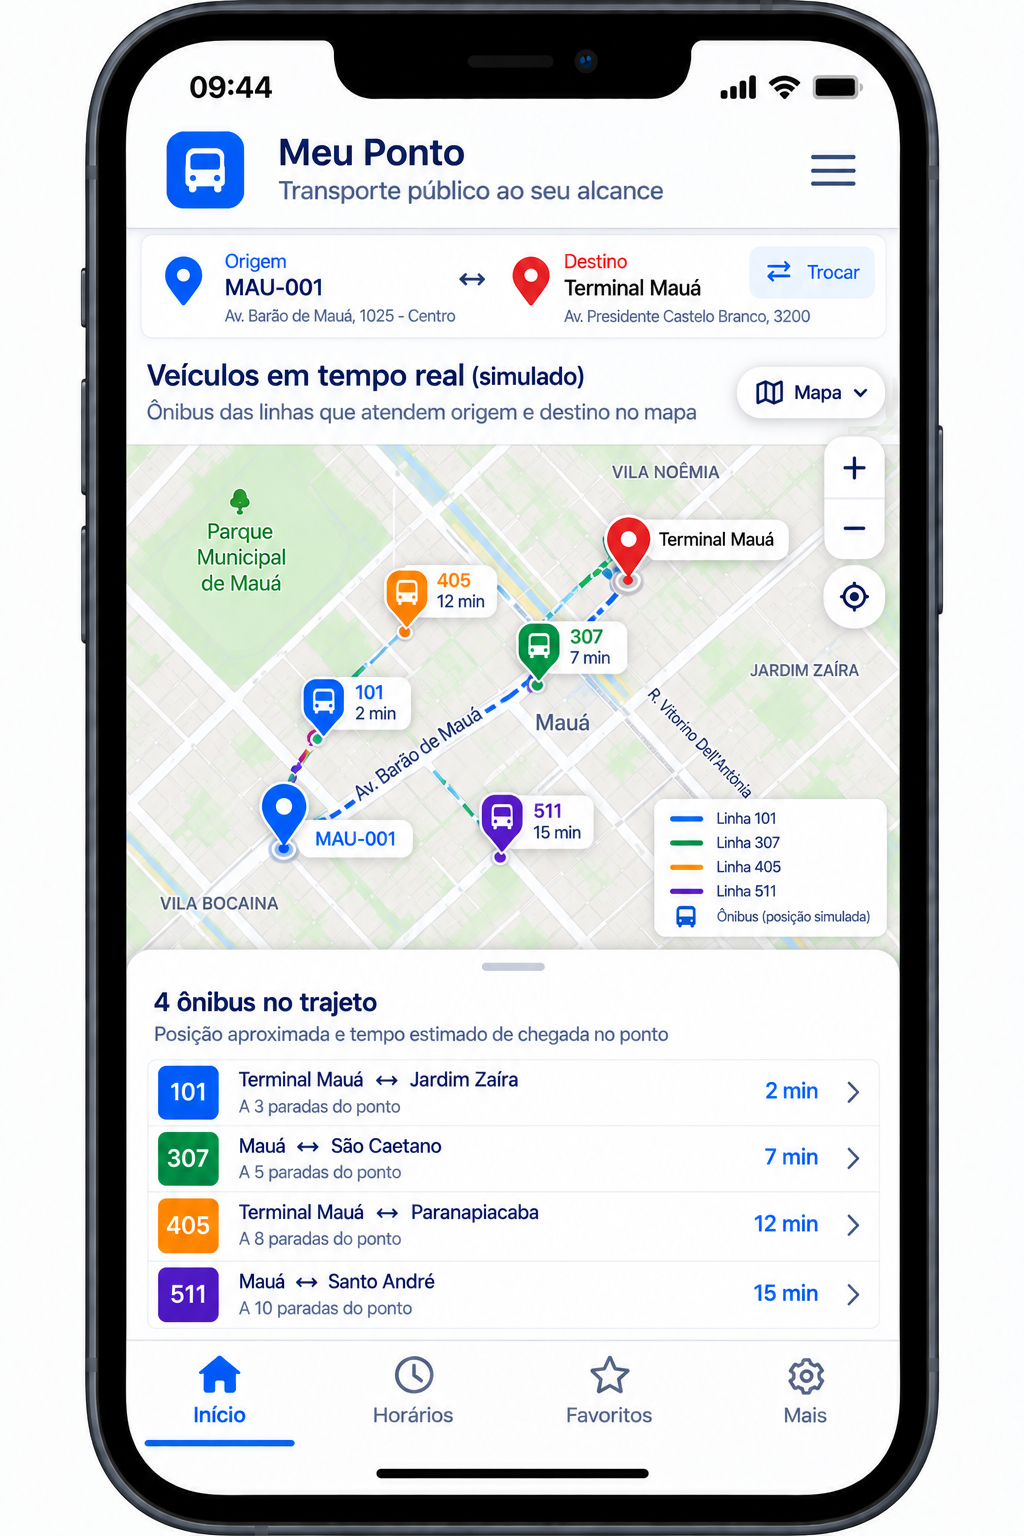
\includegraphics[width=\linewidth,height=0.52\textheight,keepaspectratio]{mockup6.png}
        \par\small (b) Veículos de diferentes linhas no mapa.
    \end{minipage}
    \caption{Mockups: filtragem por destino e acompanhamento conjunto de ônibus.}
    \label{fig:mockup-fluxo}
    \fonte{Mockups gerados automaticamente e fornecidos pelo grupo (2026); dados ilustrativos.}
\end{figure}

\clearpage
\textbf{4. Aprofundar a consulta de uma alternativa.}
O último par apresenta horários simulados, tempo estimado até o destino, mapa e sequência de paradas de uma linha selecionada (Figura~\ref{fig:mockup-detalhes}). O mapa individual é um detalhamento opcional após a comparação conjunta. A interface deverá distinguir claramente o tempo até o ônibus chegar à origem do tempo total até o passageiro alcançar o destino.

\begin{figure}[H]
    \centering
    \begin{minipage}[t]{0.48\textwidth}
        \vspace{0pt}\centering
        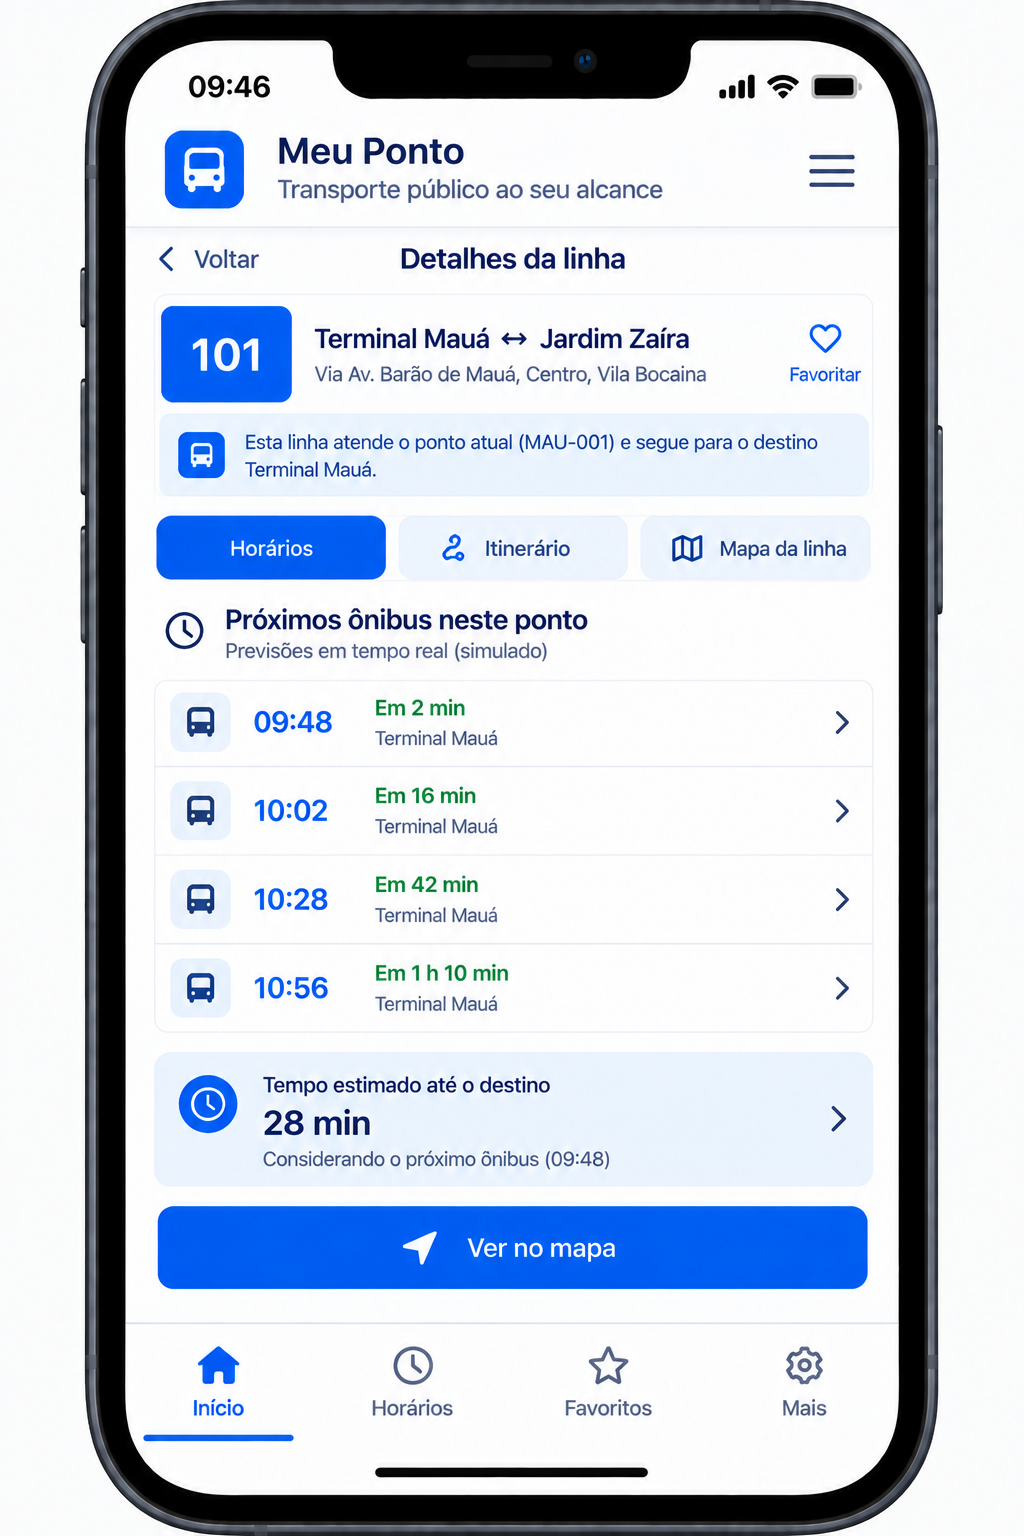
\includegraphics[width=\linewidth,height=0.52\textheight,keepaspectratio]{mockup7.png}
        \par\small (a) Horários e duração estimada da viagem.
    \end{minipage}\hfill
    \begin{minipage}[t]{0.48\textwidth}
        \vspace{0pt}\centering
        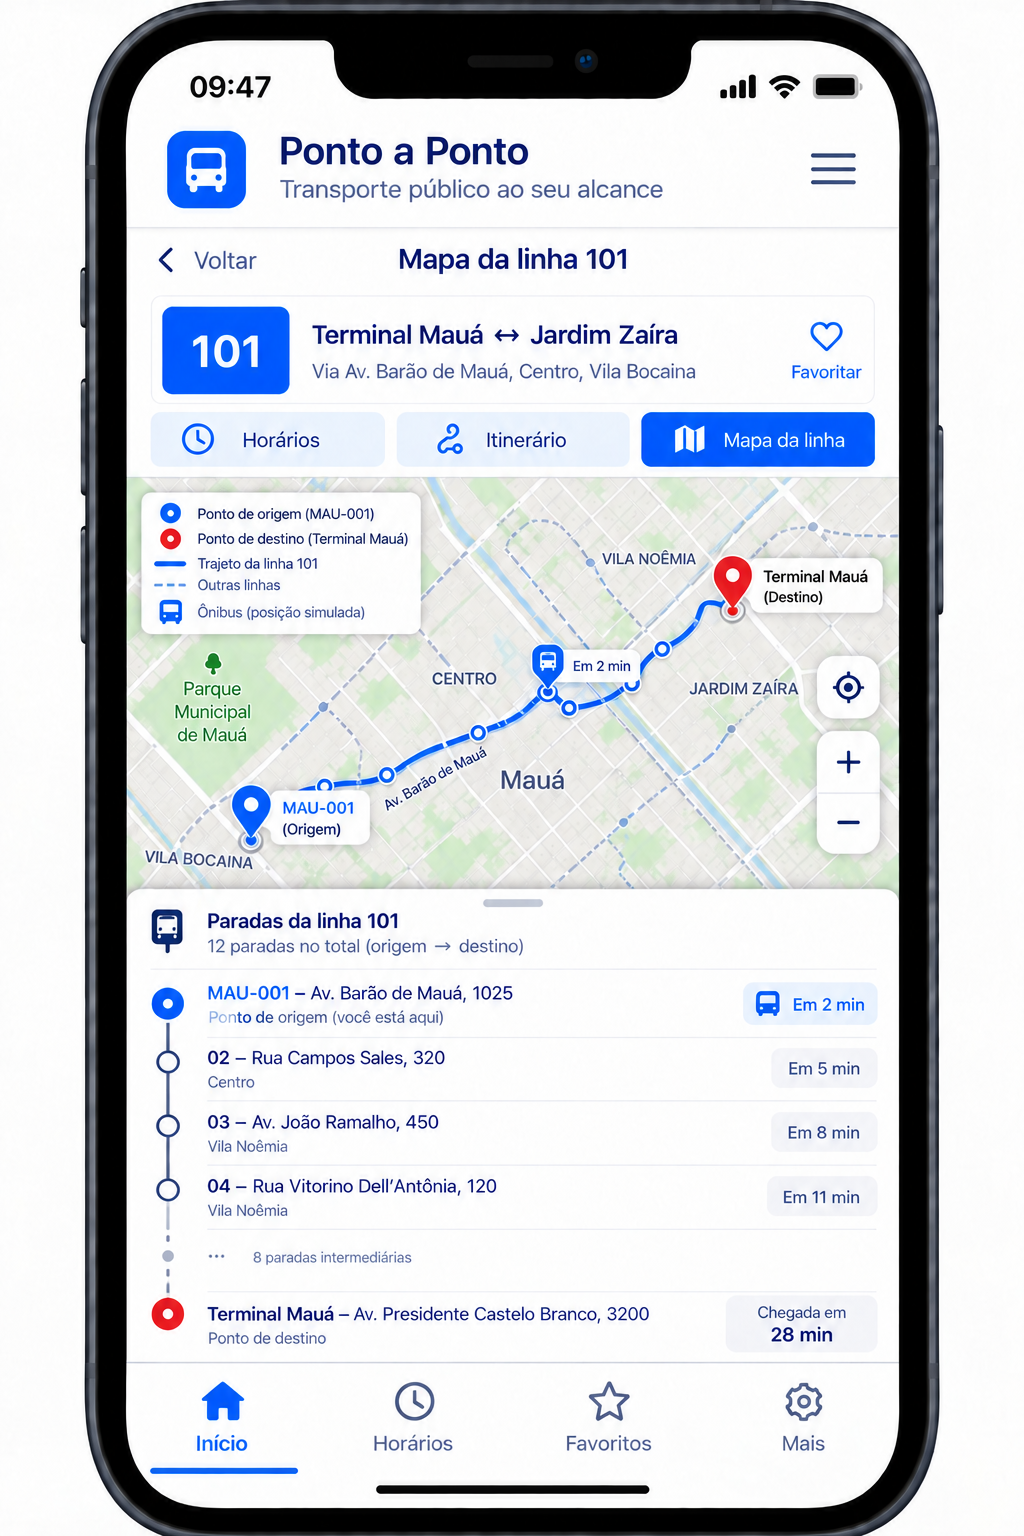
\includegraphics[width=\linewidth,height=0.52\textheight,keepaspectratio]{mockup8.png}
        \par\small (b) Trajeto e sequência de paradas.
    \end{minipage}
    \caption{Mockups: detalhes da alternativa selecionada e acompanhamento do trajeto.}
    \label{fig:mockup-detalhes}
    \fonte{Mockups gerados automaticamente e fornecidos pelo grupo (2026); dados ilustrativos.}
\end{figure}

As imagens ilustram principalmente viagens diretas e permanecem como referência conceitual. O protótipo funcional já contempla Dijkstra, baldeações no cenário e favoritos no navegador. Os valores desenhados nas telas não constituem validação numérica do algoritmo nem devem ser confundidos com os resultados da execução. A moldura de celular representa o uso web responsivo; não foi desenvolvido aplicativo Android.

\clearpage
\subsection{Seleção do destino e filtragem das alternativas}
No cenário demonstrativo, a escolha do destino aciona o cálculo das alternativas e destaca os trechos relevantes. O planejamento admite conexões que não atendem diretamente à origem e considera partidas posteriores ao veículo mais próximo. O catálogo importado permanece consultável sem que sua cobertura parcial seja tomada como rede completa apta ao cálculo.

À luz de Haylett, a evolução da interface deverá priorizar um resumo comparável das alternativas, com duração, sentido e quantidade de trocas, antes dos detalhes de cada trecho. A lista de próximas partidas deve preservar a distinção entre linha, variante e sentido, evitando que o agrupamento visual esconda diferenças de percurso. A verificação de compreensão dessas informações é parte da avaliação proposta, não um benefício já medido.

\subsection{Arquitetura implementada}
A aplicação utiliza React para seleção de origem e destino, listas, preferências locais e mapa Leaflet. Django/Python oferece a API, o planejamento, a importação e a administração. O SQLite armazena os registros utilizados na montagem dos dados da interface, sua procedência e as estimativas geográficas.

O diagrama da Figura~\ref{fig:banco-mbm}, no Apêndice~\ref{ap:importacao}, apresenta as entidades persistidas e as cardinalidades do banco. A associação entre linhas e paradas preserva a ordem do itinerário, enquanto as estimativas de localização possuem registro próprio de auditoria.

A simulação possui administração separada, com autenticação, para ativação, relógio e velocidade. O passageiro não precisa habilitá-la na tela principal. Quando desligada, veículos e previsões demonstrativas ficam indisponíveis; não há substituição automática por dados reais. O catálogo continua acessível. O isolamento dos cenários permite repetir a apresentação a Osmar e comparar o comportamento após alterações.

\subsection{Favoritos no navegador e evolução futura}
O protótipo permite salvar destinos com nomes como Casa, Trabalho e Escola, além de preferências de linhas e limite de baldeações. Os dados ficam no navegador, sem conta ou sincronização entre aparelhos. O recurso é opcional: o passageiro ocasional pode iniciar uma consulta pelo QR Code e escolher um destino no mapa sem cadastrar favoritos.

Um aplicativo Android permanece fora do escopo atual. Sua conveniência será avaliada após a validação do fluxo web, considerando necessidades que não sejam atendidas pelo navegador. A futura aplicação poderá reutilizar a API Django, mas tecnologia, distribuição e eventual sincronização ainda não foram definidas. A existência de favoritos web não depende dessa evolução.

\subsection{Objetivos da apresentação a Osmar}
A apresentação utilizará o protótipo funcional e explicitará quais informações pertencem ao cenário. Deverá discutir a utilidade do acesso sem conhecimento prévio, a comparação dos próximos ônibus e a compreensão de sentido e baldeações. O retorno profissional de Osmar será separado dos resultados de tarefas realizadas por passageiros.

Também deverão ser levantados os responsáveis e as condições de acesso ao cadastro operacional: identificadores e coordenadas de plataformas por sentido; linhas e variantes vigentes; sequência de paradas e geometrias; horários, calendários e exceções; regras de transferência; localização e previsão, quando disponíveis; periodicidade de atualização e condições de uso. O acesso a esses dados ainda não está confirmado. Qualquer piloto físico exigirá definição de responsáveis, autorização para as placas e manutenção dos QR Codes e das informações.

\subsection{Próximas etapas e limites}
As prioridades são consolidar os registros do contato inicial, apresentar o ponto-a-ponto a Osmar, executar as tarefas de compreensão com passageiros e corrigir os problemas observados. Capturas da versão efetivamente avaliada deverão complementar os mockups, com identificação da versão e do cenário. A avaliação deve verificar especialmente se o usuário reconhece a diferença entre dados reais de catálogo, coordenadas aproximadas e tempos simulados.

Em paralelo, será necessário obter e confrontar o cadastro operacional, revisar os 1.444 registros ainda sem coordenadas e validar as 30 estimativas, sem presumir corretude dos objetos OSM. Cobertura, duplicidades entre fontes, lado da via, acessibilidade de embarque, vigência e sentido precisam ser conferidos antes de habilitar planejamento real. O processo de atualização e de revisão das divergências deve preceder a substituição dos dados simulados.

O relatório registra uma implementação funcional em ambiente de demonstração. Não comprova redução de espera, precisão de chegada, cobertura integral de Mauá ou melhoria estatisticamente demonstrada da experiência do passageiro. A tese fornece fundamentos para formular requisitos e avaliar clareza; a validade desses requisitos no contexto local dependerá dos resultados da próxima etapa.

\begin{thebibliography}{99}
\bibitem{haylett2018} HAYLETT, Amanda Jane. \textit{Improving the clarity of travel information for familiar and unfamiliar travellers in public transport travel information systems}. 2018. Tese (Doctor of Engineering) -- Faculty of Engineering and the Environment, University of Southampton, Southampton, 2018.
\bibitem{mbmimportacoes} EQUIPE DO PROJETO INTEGRADOR II. \textit{ponto-a-ponto: importações externas e localização aproximada das paradas}. Documentação técnica interna do projeto, 24 set. 2026. Arquivo \texttt{docs/IMPORTACOES\_E\_GEOLOCALIZACAO.md}, manifesto \texttt{fonts/sources.json} e registros de importação do banco SQLite.
\bibitem{brakewood2019} BRAKEWOOD, C.; WATKINS, K. A literature review of the passenger benefits of real-time transit information. \textit{Transport Reviews}, v. 39, n. 3, p. 327--356, 2019. DOI: 10.1080/01441647.2018.1472147.
\bibitem{gtfs} MOBILITYDATA. \textit{General Transit Feed Specification: Overview}. Disponível em: \url{https://gtfs.org/documentation/overview/}. Acesso em: 23 set. 2026.
\bibitem{pereira2023} PEREIRA, R. H. M.; ANDRADE, P. R.; VIEIRA, J. P. B. Exploring the time geography of public transport networks with the gtfs2gps package. \textit{Journal of Geographical Systems}, v. 25, p. 453--466, 2023.
\bibitem{ma2020} MA, X. et al. Visualizing public transit system operation with GTFS data: a case study of Calgary, Canada. \textit{Heliyon}, v. 6, n. 4, e03729, 2020.
\bibitem{southampton} UNIVERSITY OF SOUTHAMPTON. \textit{Study of QR Codes in Southampton Bus Stops}. 2012. Disponível em: \url{https://blog.soton.ac.uk/data/2012/03/27/studey-of-qr-codes-in-southampton-bus-stops/}. Acesso em: 23 set. 2026.
\bibitem{hackatona2013} SÃO PAULO (Município). \textit{Hackatona do Ônibus reúne jovens para desenvolvimento de aplicativos para o transporte}. 2013. Disponível em: \url{https://prefeitura.sp.gov.br/w/noticia/hackatona-do-onibus-reune-jovens-para}. Acesso em: 23 set. 2026.
\bibitem{qrsptrans2014} SÃO PAULO (Município). \textit{Nova tecnologia, QR Code já fornece informações por celular aos usuários de ônibus}. 24 jun. 2014. Disponível em: \url{https://prefeitura.sp.gov.br/web/mobilidade/w/noticias/173515}. Acesso em: 23 set. 2026.
\bibitem{sptransparada70016782} SÃO PAULO TRANSPORTE S.A. \textit{Informações desta parada: Av. Paulista, n. 200, código 70016782}. Disponível em: \url{http://qrcodeadesivo.extapps.sptrans.com.br/QRCodeAdesivo/adesivo.aspx?70016782}. Acesso em: 23 set. 2026.
\bibitem{sptransadesivojs} SÃO PAULO TRANSPORTE S.A. \textit{Aplicação QRCodeAdesivo: adesivo.js}. Recurso público; cabeçalho HTTP Last-Modified consultado. Disponível em: \url{http://qrcodeadesivo.extapps.sptrans.com.br/QRCodeAdesivo/adesivo.js?2021631733832}. Acesso em: 23 set. 2026.
\bibitem{sptransgxcfg} SÃO PAULO TRANSPORTE S.A. \textit{Aplicação QRCodeAdesivo: gxcfg.js}. Recurso público; cabeçalho HTTP Last-Modified consultado. Disponível em: \url{http://qrcodeadesivo.extapps.sptrans.com.br/QRCodeAdesivo/gxcfg.js?54798}. Acesso em: 23 set. 2026.
\bibitem{sptranscss} SÃO PAULO TRANSPORTE S.A. \textit{Aplicação QRCodeAdesivo: GeneXusXEv2.css}. Recurso público; cabeçalho HTTP Last-Modified consultado. Disponível em: \url{http://qrcodeadesivo.extapps.sptrans.com.br/QRCodeAdesivo/Resources/Portuguese/GeneXusXEv2.css?14585136}. Acesso em: 23 set. 2026.
\bibitem{sptransgxgral} SÃO PAULO TRANSPORTE S.A. \textit{Aplicação QRCodeAdesivo: gxgral.js}. Recurso público; cabeçalho HTTP Last-Modified consultado. Disponível em: \url{http://qrcodeadesivo.extapps.sptrans.com.br/QRCodeAdesivo/gxgral.js?54798}. Acesso em: 23 set. 2026.
\bibitem{sptransapi} SÃO PAULO TRANSPORTE S.A. \textit{API do Olho Vivo: guia de referência}. Disponível em: \url{https://www.sptrans.com.br/desenvolvedores/api-do-olho-vivo-guia-de-referencia/documentacao-api/}. Acesso em: 23 set. 2026.
\bibitem{osmlicense} OPENSTREETMAP FOUNDATION. \textit{Direitos autorais e licença}. Disponível em: \url{https://www.openstreetmap.org/copyright?locale=pt}. Acesso em: 23 set. 2026.
\bibitem{osmpt} OPENSTREETMAP WIKI. \textit{Key:public transport}. Disponível em: \url{https://wiki.openstreetmap.org/wiki/Key:public_transport}. Acesso em: 23 set. 2026.
\bibitem{overpass} OPENSTREETMAP WIKI. \textit{Overpass API}. Disponível em: \url{https://wiki.openstreetmap.org/wiki/Overpass_API}. Acesso em: 23 set. 2026.
\bibitem{geolocation} MDN WEB DOCS. \textit{Geolocation API}. Disponível em: \url{https://developer.mozilla.org/en-US/docs/Web/API/Geolocation_API}. Acesso em: 23 set. 2026.
\bibitem{responsive} MDN WEB DOCS. \textit{Responsive web design}. Disponível em: \url{https://developer.mozilla.org/en-US/docs/Learn_web_development/Core/CSS_layout/Responsive_Design}. Acesso em: 23 set. 2026.
\bibitem{react} REACT. \textit{React documentation}. Disponível em: \url{https://react.dev/}. Acesso em: 23 set. 2026.
\bibitem{django} DJANGO SOFTWARE FOUNDATION. \textit{Django documentation}. Disponível em: \url{https://docs.djangoproject.com/en/6.0/}. Acesso em: 23 set. 2026.
\bibitem{postgis} POSTGIS PROJECT. \textit{PostGIS Manual}. Disponível em: \url{https://postgis.net/docs/en/}. Acesso em: 23 set. 2026.
\bibitem{sedgewicksp} SEDGEWICK, R.; WAYNE, K. \textit{Algorithms, 4th edition: 4.4 Shortest Paths}. Disponível em: \url{https://algs4.cs.princeton.edu/44sp/}. Acesso em: 23 set. 2026.
\bibitem{transitplanner} UNIVERSITÄT FREIBURG. \textit{Transit Planner: Basic Concepts}. Disponível em: \url{https://ad-publications.cs.uni-freiburg.de/student-projects/transfer-patterns-robustness/concepts.html}. Acesso em: 23 set. 2026.
\bibitem{git} CHACON, S.; STRAUB, B. \textit{Pro Git}. 2. ed. Disponível em: \url{https://git-scm.com/book/pt-br/v2}. Acesso em: 23 set. 2026.
\end{thebibliography}

\begin{apendicesenv}
\chapter{Conversão e geolocalização dos dados}
\label{ap:importacao}
Este apêndice descreve a implementação registrada em 24 de setembro de 2026, em complemento à Seção~\ref{sec:conversao}. Os parâmetros são heurísticos da versão \nolinkurl{osm-address-directed-v1.1}; não representam percentuais de acerto nem calibração com a operadora. Código e documentação interna permanecem como registro técnico de apoio \cite{mbmimportacoes}.

\section*{A.1 Mapeamento para o SQLite}
\begingroup\small
\setlength{\tabcolsep}{4pt}
\setlength{\parskip}{0pt}
\begin{longtable}{>{\raggedright\arraybackslash}p{0.29\textwidth}>{\raggedright\arraybackslash}p{0.66\textwidth}}
\caption{Correspondência entre dados importados e modelos Django}\label{tab:modelos-importacao}\\
\hline Modelo & Campos e responsabilidade \\\hline
\endfirsthead
\hline Modelo & Campos e responsabilidade (continuação) \\\hline
\endhead
\hline\endfoot
\texttt{SourceDocument} & \texttt{id}, \texttt{provider}, \texttt{url}, \texttt{kind}, \texttt{status}, \texttt{metadata}, \texttt{content} e \texttt{imported\_at}: origem, estado da coleta, hash, datas e texto extraído. A data de importação não é a data de vigência do serviço.\\
\texttt{Stop} & \texttt{id}, \texttt{name}, \texttt{lat}, \texttt{lon}, \texttt{source} e \texttt{data}: identificação, endereço e atributos originais, coordenadas opcionais e situação da geolocalização. Ausência de coordenadas é representada por valor nulo.\\
\texttt{Route} & \texttt{id}, \texttt{code}, \texttt{name}, \texttt{source}, \texttt{simulated}, \texttt{routable} e \texttt{data}: variante e procedência. Horários documentais e itinerários textuais permanecem em dados complementares; \texttt{simulated} distingue os cenários.\\
\texttt{RouteStop} & \texttt{route}, \texttt{stop}, \texttt{position}, \texttt{duration} e \texttt{segment}: ocorrência da parada na sequência, duração e geometria do segmento quando disponíveis. A unicidade é por variante e posição, permitindo repetição do mesmo ID ao longo do percurso.\\
\texttt{NetworkMetadata} & \texttt{name} e \texttt{data}: parâmetros complementares da rede demonstrativa, como origem padrão e configuração do cenário.\\
\texttt{GeolocationRun} & \texttt{created\_at}, \texttt{algorithm}, \texttt{source\_hash} e \texttt{summary}: versão, entrada e resultado resumido da execução.\\
\texttt{StopEstimate} & \texttt{route}, \texttt{stop}, \texttt{position}, \texttt{run}, \texttt{status}, \texttt{lat}, \texttt{lon} e \texttt{evidence}: decisão e evidências por ocorrência; coordenadas hipotéticas de uma pendência não são publicadas como posição da parada.\\
\end{longtable}
\endgroup

Uma variante é marcada como roteável na importação quando possui pelo menos duas paradas, coordenadas para todas elas e durações consistentes; nesse caso também se exige intervalo positivo entre viagens. Esse teste técnico não certifica itinerário autorizado, calendário vigente ou geometria adequada para ônibus. As variantes públicas incompletas permanecem disponíveis no catálogo, separadas do cenário de planejamento.

Os registros são atualizados por identificadores estáveis. Uma nova importação com o mesmo endereço e sem coordenada própria preserva a estimativa existente; alteração de endereço invalida a estimativa associada. Mudança de sequência invalida as estimativas da variante e as posições derivadas afetadas, exigindo novo processamento. A mera ausência de um registro na coleta não aciona exclusão automática nem comprova desativação do serviço.


\clearpage
\begin{figure}[p]
\centering
\caption{Diagrama do banco de dados de domínio do ponto-a-ponto}
\label{fig:banco-mbm}
\resizebox{\textwidth}{!}{% Diagrama vetorial do esquema de domínio do MBM, conferido no SQLite.
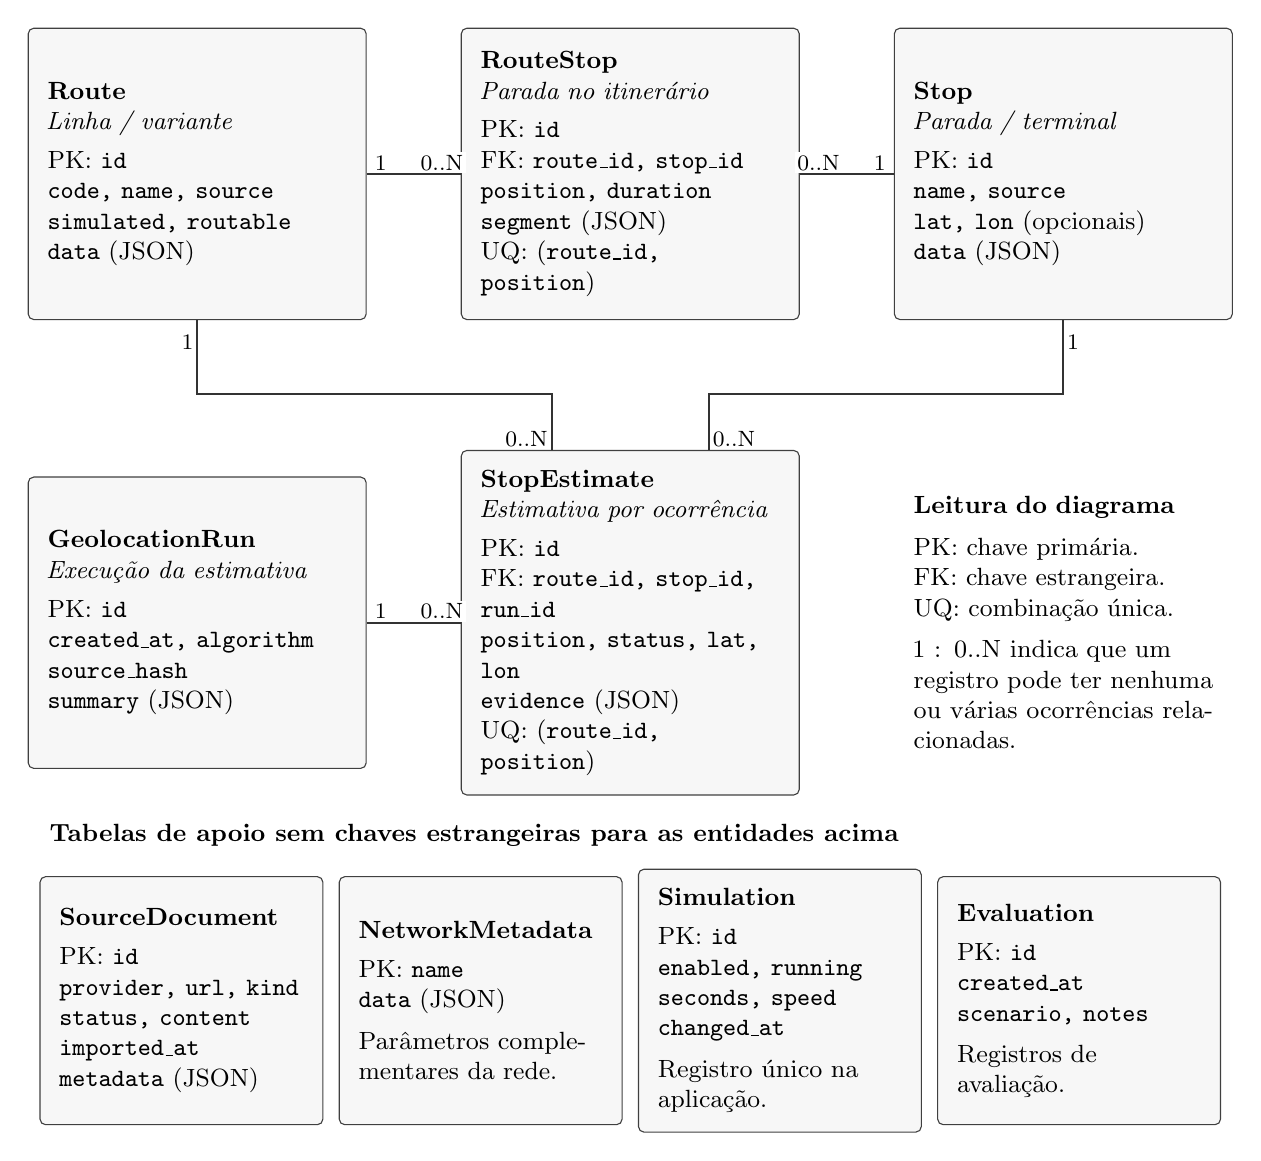
\begin{tikzpicture}[
  entity/.style={draw=black!75, fill=black!3, rounded corners=2pt,
    text width=3.8cm, inner sep=7pt, align=left, font=\fontsize{9}{11}\selectfont},
  support/.style={entity, text width=3.1cm, minimum height=3.15cm},
  relation/.style={draw=black!80, line width=0.7pt},
  cardinal/.style={font=\fontsize{8}{10}\selectfont, fill=white, inner sep=1pt}
]
\node[entity, minimum height=3.7cm] (route) at (0,0) {
  \textbf{Route}\\\textit{Linha / variante}\\[3pt]
  PK: \texttt{id}\\
  \texttt{code, name, source}\\
  \texttt{simulated, routable}\\
  \texttt{data} (JSON)
};
\node[entity, minimum height=3.7cm] (rs) at (5.5,0) {
  \textbf{RouteStop}\\\textit{Parada no itinerário}\\[3pt]
  PK: \texttt{id}\\
  FK: \texttt{route\_id, stop\_id}\\
  \texttt{position, duration}\\
  \texttt{segment} (JSON)\\
  UQ: (\texttt{route\_id, position})
};
\node[entity, minimum height=3.7cm] (stop) at (11,0) {
  \textbf{Stop}\\\textit{Parada / terminal}\\[3pt]
  PK: \texttt{id}\\
  \texttt{name, source}\\
  \texttt{lat, lon} (opcionais)\\
  \texttt{data} (JSON)
};
\node[entity, minimum height=3.7cm] (run) at (0,-5.7) {
  \textbf{GeolocationRun}\\\textit{Execução da estimativa}\\[3pt]
  PK: \texttt{id}\\
  \texttt{created\_at, algorithm}\\
  \texttt{source\_hash}\\
  \texttt{summary} (JSON)
};
\node[entity, minimum height=3.7cm] (estimate) at (5.5,-5.7) {
  \textbf{StopEstimate}\\\textit{Estimativa por ocorrência}\\[3pt]
  PK: \texttt{id}\\
  FK: \texttt{route\_id, stop\_id,}\\
  \texttt{run\_id}\\
  \texttt{position, status, lat, lon}\\
  \texttt{evidence} (JSON)\\
  UQ: (\texttt{route\_id, position})
};
\draw[relation] (route.east) -- node[cardinal,above,pos=.15]{1}
  node[cardinal,above,pos=.8]{0..N} (rs.west);
\draw[relation] (stop.west) -- node[cardinal,above,pos=.15]{1}
  node[cardinal,above,pos=.8]{0..N} (rs.east);
\draw[relation] (run.east) -- node[cardinal,above,pos=.15]{1}
  node[cardinal,above,pos=.8]{0..N} (estimate.west);
\draw[relation] (route.south) -- node[cardinal,left,pos=.3]{1}
  (0,-2.8) -- (4.5,-2.8) -- node[cardinal,left,pos=.8]{0..N}
  ([xshift=-1cm]estimate.north);
\draw[relation] (stop.south) -- node[cardinal,right,pos=.3]{1}
  (11,-2.8) -- (6.5,-2.8) -- node[cardinal,right,pos=.8]{0..N}
  ([xshift=1cm]estimate.north);
\node[align=left,text width=3.8cm,font=\fontsize{9}{11}\selectfont] at (11,-5.7) {
  \textbf{Leitura do diagrama}\\[4pt]
  PK: chave primária.\\
  FK: chave estrangeira.\\
  UQ: combinação única.\\[4pt]
  1 : 0..N indica que um registro pode ter nenhuma ou várias ocorrências relacionadas.
};
\node[font=\fontsize{9}{11}\selectfont\bfseries,anchor=west] at (-2,-8.4) {Tabelas de apoio sem chaves estrangeiras para as entidades acima};
\node[support] at (-.2,-10.5) {
  \textbf{SourceDocument}\\[3pt]
  PK: \texttt{id}\\
  \texttt{provider, url, kind}\\
  \texttt{status, content}\\
  \texttt{imported\_at}\\
  \texttt{metadata} (JSON)
};
\node[support] at (3.6,-10.5) {
  \textbf{NetworkMetadata}\\[3pt]
  PK: \texttt{name}\\
  \texttt{data} (JSON)\\[4pt]
  Parâmetros complementares da rede.
};
\node[support] at (7.4,-10.5) {
  \textbf{Simulation}\\[3pt]
  PK: \texttt{id}\\
  \texttt{enabled, running}\\
  \texttt{seconds, speed}\\
  \texttt{changed\_at}\\[4pt]
  Registro único na aplicação.
};
\node[support] at (11.2,-10.5) {
  \textbf{Evaluation}\\[3pt]
  PK: \texttt{id}\\
  \texttt{created\_at}\\
  \texttt{scenario, notes}\\[4pt]
  Registros de avaliação.
};
\end{tikzpicture}
}
\fonte{Elaboração do grupo a partir dos modelos Django e do esquema SQLite do ponto-a-ponto, conferidos em 24 set. 2026.}
\end{figure}
\clearpage

A Figura~\ref{fig:banco-mbm} representa as nove tabelas de domínio pelos nomes dos modelos Django; no SQLite, seus nomes recebem o prefixo \texttt{transit\_}. As tabelas internas de autenticação, sessões, permissões e migrações do Django foram omitidas para concentrar a leitura no projeto. São indicadas as chaves primárias, estrangeiras e a unicidade de variante e posição em \texttt{RouteStop} e de execução, variante e posição em \texttt{StopEstimate}.

\texttt{RouteStop} implementa a associação muitos-para-muitos entre \texttt{Route} e \texttt{Stop}, acrescentando ordem, duração e geometria do segmento. Uma linha pode repetir a mesma parada em posições diferentes. \texttt{StopEstimate} associa uma ocorrência a uma linha, a uma parada e à execução que produziu sua estimativa. Embora represente a mesma combinação de variante e posição do itinerário, não possui chave estrangeira direta para \texttt{RouteStop}; essa correspondência é mantida pela aplicação.

\texttt{SourceDocument} guarda a procedência documental, mas não possui uma chave estrangeira que o ligue diretamente às paradas ou linhas. O vínculo de procedência é registrado pelos identificadores de fonte, URLs e metadados. Por isso, o diagrama não desenha relações referenciais inexistentes. \texttt{NetworkMetadata}, \texttt{Simulation} e \texttt{Evaluation} também são independentes das entidades da rede no esquema relacional. A presença da tabela de avaliações não implica que já tenha ocorrido avaliação com a comunidade.

\section*{A.2 Entradas e construção de candidatos}
A consulta viária cobre o retângulo de latitude/longitude \texttt{(-23.74, -46.54, -23.60, -46.39)}, incluindo áreas vizinhas. O recorte coletado em 24/09/2026 contém 26.393 objetos, dos quais o índice aproveitou 2.385 endereços numerados. A resposta declara data-base de 15/07/2026 às 15:22:01 UTC. Preservam-se a resposta original, os metadados e o hash; uma nova coleta poderá produzir outro resultado.

A normalização remove acentos e pontuação e expande abreviações de logradouros. Mantém-se o texto original para auditoria. Um intervalo numérico, como 4019--4075, usa o ponto médio 4047 apenas como hipótese. A busca considera \texttt{name}, \texttt{alt\_name} e \texttt{short\_name}; sem coincidência exata, exige similaridade mínima de 0,90 e vantagem de 0,05 sobre o segundo nome candidato. Quando a cidade está explicitada nas duas entradas, ela deve concordar.

Prioriza-se uma âncora com rua e número exatos. Para um edifício poligonal, a média dos vértices disponíveis é uma referência aproximada, não sua entrada física. Sem número exato, interpola-se entre números inferior e superior da mesma rua somente se as âncoras estiverem a até 500 metros entre si e a diferença numérica for no máximo 1.000. Não há extrapolação nem inferência de paridade de calçadas. As regras especiais de objetos OSM \texttt{addr:interpolation} não são interpretadas nesta versão.

Para projetar uma referência $P$ no segmento de rua $A\rightarrow B$, em coordenadas métricas locais, utiliza-se:
\[
 t=\min\left(1,\max\left(0,\frac{(P-A)\cdot(B-A)}{\lVert B-A\rVert^2}\right)\right),
 \qquad Q=A+t(B-A).
\]
A conversão planar usa 111.320 metros por grau de latitude e o cosseno da latitude de referência $-23{,}67^\circ$ para longitude. Aceitam-se projeções a até 100 metros da referência e retêm-se até quatro alternativas próximas. Sem âncoras numéricas, são geradas cinco hipóteses distribuídas pelo comprimento acumulado da rua, sem publicação automática.

\section*{A.3 Sentido, conectividade e custo}
O grafo viário utiliza nós compartilhados e sentidos permitidos; proximidade visual não cria conexão. A regra \texttt{oneway=-1} inverte a orientação; \texttt{oneway:bus} e \texttt{oneway:psv} podem alterar a regra geral. Proibições explícitas para ônibus e acessos privados sem exceção são filtrados. Regras condicionais reconhecidas são excluídas, pois esta versão não avalia calendário operacional. Relações OSM de restrição de conversão não são interpretadas, o que limita a validade operacional dos caminhos.

A distância dirigida entre candidatos usa A* com heurística euclidiana e limite de busca de oito quilômetros entre nós. Frações dos segmentos nas projeções são consideradas; movimento para trás em uma via de mão única não é aceito como ligação direta. A ordem publicada das paradas orienta a inferência, e não nomes como Centro/Bairro ou o crescimento da numeração dos imóveis.

A programação dinâmica seleciona uma sequência de candidatos minimizando:
\[
 F_t(c)=L(c)+\min_p\left[F_{t-1}(p)+\frac{d_{\mathrm{dir}}(p,c)}{150}\right],
 \qquad L(c)=\frac{d_{\mathrm{proj}}(c)}{30}+\eta(c).
\]
As distâncias são expressas em metros; $\eta=1$ para correspondência textual aproximada e $\eta=0$ para exata. Os divisores são escalas heurísticas de custo, não velocidades. O procedimento escolhe hipóteses de localização e não calcula tempo de viagem. Uma parada sem candidatos divide a sequência em blocos; não se salta essa lacuna para fabricar conectividade. Blocos sem caminho dirigido permanecem pendentes. Dijkstra, empregado no planejamento demonstrativo de passageiros, é uma etapa distinta.

\section*{A.4 Aceitação, conciliação e auditoria}
A ambiguidade é avaliada comparando a solução com alternativas a mais de 40 metros ou com diferença angular superior a $45^\circ$. Uma referência numérica exige margem de custo de pelo menos 0,5. Sem referência numérica própria, exige-se margem de pelo menos 1,0 e apoio de ao menos uma referência numérica entre as duas posições anteriores e outra entre as duas posteriores do bloco.

Aplica-se deslocamento de três metros à direita do sentido inferido. Essa hipótese não mede largura da pista, calçada ou abrigo; embarque à esquerda, ilhas centrais e terminais requerem revisão. Guardam-se ponto no eixo, posição deslocada, azimute, ID da via, âncoras, método, margem e motivo da decisão.

As estimativas aceitas do mesmo ID são comparadas entre variantes. Discordância máxima superior a 60 metros ou diferença de sentido superior a $90^\circ$ impede publicar uma posição consensual. Caso contrário, escolhe-se o medoide, isto é, a posição calculada cuja soma das distâncias às demais é mínima. IDs diferentes não são fundidos por esse procedimento.

Os estados são \texttt{estimated}, \texttt{pending} e \texttt{conflict}. O estado \texttt{validated} exige revisão humana registrada com responsável, data e evidência; o algoritmo nunca o atribui. Na interface, a estimativa recebe contorno tracejado e indicação de posição aproximada. A execução \texttt{run-2} aceitou 272 ocorrências: quatro por número exato, 194 por interpolação e 74 por hipóteses apoiadas na sequência. A conciliação resultou em 30 IDs publicados. Das 3.463 ocorrências pendentes, 575 apresentaram rua ausente ou ambígua, 2.626 apresentaram ambiguidade de endereço/sentido e 262 não tiveram continuidade dirigida dentro dos limites da busca.

\section*{A.5 Reprodução e conservação das evidências}
Na raiz do ponto-a-ponto, com as dependências instaladas e o ambiente Python ativo, a reprodução a partir das entradas preservadas utiliza:
\begin{verbatim}
python backend/manage.py migrate
python backend/manage.py import_sources
python backend/manage.py geolocate_stops
\end{verbatim}
O primeiro importador utiliza os arquivos locais existentes; o geolocalizador utiliza o recorte viário preservado. Para coletar novamente, os comandos são:
\begin{verbatim}
python backend/manage.py import_sources --download
python backend/manage.py geolocate_stops --download
\end{verbatim}
O coletor pode reutilizar o cache; \texttt{import\_sources --download --refresh} solicita atualização das respostas. A opção \texttt{--demo} do importador acrescenta explicitamente as seis linhas simuladas. Para examinar apenas uma variante:
\begin{verbatim}
python backend/manage.py geolocate_stops \
  --route cittamobi:169f6fbfd86b
\end{verbatim}
A execução parcial é estritamente diagnóstica: registra evidências sem alterar coordenadas publicadas ou estimativas exibidas no catálogo. A conciliação da rede exige execução completa e utiliza apenas as estimativas dessa execução. Reexecuções e reimportações preservam as evidências históricas; a unicidade das estimativas inclui execução, variante e posição. Para reproduzir os números apresentados, é necessário conservar a versão do código e as mesmas entradas: manifesto, respostas em \texttt{fonts/raw/}, \texttt{fonts/collected.json}, \texttt{fonts/osm.json}, consulta e resposta viária, metadados e hashes. Os relatórios ficam em \nolinkurl{fonts/geolocation_runs/run-<id>.json}; as tabelas de auditoria também registram a execução. Arquivos volumosos não são todos versionados no Git, e uma nova coleta não garante os mesmos resultados.

A administração permite consultar execuções e estimativas e registrar revisões humanas. A inspeção do lado de embarque, vigência, acessibilidade, sentidos e itinerários autorizados permanece necessária antes de uso operacional. O cadastro importado e este método aproximativo não substituem o cadastro da operadora ou uma verificação de campo.
\end{apendicesenv}

\end{document}
